\documentclass[format=acmsmall,authorversion]{acmart}

\makeatletter
\def\@ACM@checkaffil{% Only warnings
    \if@ACM@instpresent\else
    \ClassWarningNoLine{\@classname}{No institution present for an affiliation}%
    \fi
    \if@ACM@citypresent\else
    \ClassWarningNoLine{\@classname}{No city present for an affiliation}%
    \fi
    \if@ACM@countrypresent\else
        \ClassWarningNoLine{\@classname}{No country present for an affiliation}%
    \fi
}
\makeatother                                        

\settopmatter{printacmref=false} % Removes citation information below abstract
\renewcommand\footnotetextcopyrightpermission[1]{} % removes footnote with conference information in first column
\pagestyle{plain} % removes running headers
\usepackage{acm-ec-24}
\usepackage{booktabs} % For formal tables
\usepackage[ruled]{algorithm2e} % For algorithms
\renewcommand{\algorithmcfname}{ALGORITHM}
\SetAlFnt{\small}
\SetAlCapFnt{\small}
\SetAlCapNameFnt{\small}
\SetAlCapHSkip{0pt}
\IncMargin{-\parindent}

% Choose a citation style by commenting/uncommenting the appropriate line:
\setcitestyle{acmnumeric}
% \setcitestyle{authoryear}



\usepackage{graphicx}
\usepackage{mathtools,amsfonts}
\usepackage{array}
\usepackage{multirow, hhline}
\usepackage{paralist}

\usepackage{algpseudocode}
% \usepackage[usenames,dvipsnames,table]{xcolor}
\usepackage{xcolor}
\usepackage{wrapfig}
\usepackage[english]{babel}		% Allows hiphenization of words and other stuff
% \usepackage[margin=1in]{geometry}	% Defines margins to 1 inch
\usepackage{geometry}
\usepackage{lipsum}			% provides filler text \lipsum[n]
\usepackage{comment}
\usepackage{chngpage}			% Allows width to be changed dynamically
\usepackage{amsfonts,amsmath, amsthm}
\usepackage{amsopn}
\usepackage{color}
\usepackage{blindtext}
\usepackage{multicol}
\usepackage{amsmath}
\usepackage{color}


\usepackage{pgfplots}
\usepackage{pgfgantt}
%\pgfplotsset{compat=1.15}
\usepackage{tikz}
\usetikzlibrary{arrows}
\usetikzlibrary{calc}
\usepackage{algpseudocode}
%\usepackage{algorithmicx}
%\usepackage[noend]{algcompatible}
% \usepackage[Algorithm]{algorithm}
\usepackage{subcaption}
%\usepackage[Algorithm]{algorithm2e}
\usepackage{tabto}
\usepackage{csquotes} %quotations
\usepackage{multirow}
\usepackage{amsthm}

\fancyfoot{}
% \usepackage{fancyhdr}
% \AtBeginDocument{%
%     \addtolength{\footskip}{2.0\baselineskip}%
%     \fancyfoot[L]{\textit{\textbf{Preprint --- do not distribute.}}}%
% }

% Links nas refs e bookmarks
% \usepackage[colorlinks,urlcolor=black,citecolor=black,linkcolor=black,menucolor=black]{hyperref}
\usepackage{hyperref}
\usepackage[capitalise]{cleveref} 
\newcommand\pcref[1]{(\cref{#1})}

\crefname{enumi}{}{}

\setlength{\columnseprule}{1pt}
\def\columnseprulecolor{\color{black}}

% \graphicspath{ {./plots/} }

% --- Paragraph formatting ---
% \usepackage{parskip} 				% Allows paragraphs to have spacing
% \usepackage{indentfirst}			% Indents first paragraph
% \usepackage{titlesec}				% Allows control of spacing on sections and paragraphs
% \setlength{\parindent}{0.25in} 			% Sets the indent
% \setlength{\parskip}{3pt}			% Sets the spacing
% \titlespacing{\paragraph}{%
%   0pt}{%              left margin
%   0.5\baselineskip}{% space before (vertical)
%   1em}%               space after (horizontal)

\newtheorem{theorem}{Theorem}
\newtheorem*{theorem*}{Theorem}
\newtheorem{acknowledgment}[theorem]{Acknowledgment}
\newtheorem{corollary}[theorem]{Corollary}
\newtheorem{definition}[theorem]{Definition}
\newtheorem{remark}[theorem]{Remark}
\newtheorem{lemma}[theorem]{Lemma}
\newtheorem{problem}[theorem]{Problem}
\newtheorem{fact}[theorem]{Fact}
\newtheorem{proposition}[theorem]{Proposition}
\newtheorem{observation}[theorem]{Observation}
\newtheorem{claim}[theorem]{Claim}
\newtheorem{conjecture}[theorem]{Conjecture}
% \let\doendproof\endproof
% \renewcommand\endproof{~\hfill\qed\doendproof}
\newcommand{\GMMS}{\mathit{GMMS}}
\newcommand{\MMS}{\mathit{MMS}}
\newcommand{\mea}{\mathit{mea}}
\newcommand{\DM}{\mathit{DM}}
\newcommand{\EFX}{\mathit{EFX'}}
\newcommand{\DGM}{\mathit{DGM}}
\newcommand{\UM}{\mathit{UM}}
\newcommand{\block}{\mathit{block}}
\newcommand{\argmin}[1]{\underset{#1}{\operatorname{\mathrm{arg\,max}}}}
\newcommand{\argmax}{{\operatorname{\mathrm{arg\,max}}}}
\newcommand{\argmaxKM}{\operatorname{arg\,max}}
\newcommand{\bigOsymb}{\ensuremath{\mathcal{O}}}
\newcommand{\bigO}[1]{\ensuremath{\mathcal{O}\left(#1\right)}}
%\newcommand{\eps}{\texorpdfstring{\ensuremath{\varepsilon^{5}}}{epsilon}}
\newcommand{\norm}[1]{\lvert\lvert #1 \rvert\rvert}
\newcommand{\red}[1]{{\color{blue!90!black} #1}}
\newcommand{\abs}[1]{| #1 |}
\newcommand{\set}[2]{ \{ #1 \; | \; #2 \} }
\newcommand{\sset}[1]{\left\{ #1 \right\} } 
\newcommand{\R}{\mathbb{R}}

\newcommand{\cD}{\mathcal{D}}
\newcommand{\bbR}{\mathbb{R}} 

\DeclarePairedDelimiterX{\inp}[2]{\langle}{\rangle}{#1, #2}
\DeclarePairedDelimiterX{\cb}[1]{\{}{\}}{#1}
%\DeclareMathOperator*{\argmin}{arg\,min}


\newcommand{\lref}[1]{(\ref{#1})}
\newcommand{\KM}[1]{{\textcolor{blue}{#1}}}
\newcommand{\KMtwo}[2]{{\tiny \textcolor{green}{#1}}\textcolor{blue}{#2}}
\newcommand{\BRC}[1]{{\textcolor{red}{BRC: #1}}}
\newcommand{\ck}[1]{{\textcolor{red}{CK: #1}}}
\newcommand{\ntl}[1]{{\textcolor{teal}{Tianlong: #1}}}
\newcommand{\notename}[2]{{\textcolor{blue}{\footnotesize{\bf (#1:} {#2}{\bf ) }}}}
\newcommand{\RM}[1]{{\notename{RM}{#1}}}
\newcommand{\rmedit}[1]{{\textcolor{purple}{#1}}}


\newcommand{\myBox}[3]{\begin{array}{|c|} \hline #1 \\ \hline #2 \\ \hline  \multicolumn{1}{c}{} \\[-0.7em] \multicolumn{1}{c}{(#3)} \end{array}}
\newcommand{\myBoxtwo}[2]{\begin{array}{|c|} \hline \\ {\raisebox{0.5em}[0cm][0cm]{\ensuremath{#1}}} \\ \hline \multicolumn{1}{c}{} \\[-0.7em]\multicolumn{1}{c}{(#2)} \end{array}}


%\newcommand{\myBox}[3]{$\begin{array}{|c|} \hline #1 \\ \hline #2 \\ \hline \multicolumn{1}{c}{}\\ \multicolumn{1}{c}{(#3)} \end{array}$}
%\newcommand{\myBoxtwo}[2]{$\begin{array}{|c|} \hline #1 \\        \\ \hline \multicolumn{1}{c}{}\\ \multicolumn{1}{c}{(#2)} \end{array}$}



\newcommand{\Allocation}[6]{\myBox{#1}{#2}{1}\hspace{2em}\myBox{#3}{#4}{2}\hspace{2em}\myBox{#5}{#6}{3}}
\newcommand{\Allocationfive}[5]{\myBox{#1}{#2}{1}\hspace{2em}\myBox{#3}{#4}{2}\hspace{2em}\myBoxtwo{#5}{3}}
\newcommand{\Allocationfivetwo}[5]{\myBox{#1}{#2}{1}\hspace{2em}\myBoxtwo{#3}{2}\hspace{2em}\myBox{#4}{#5}{3}}
\newcommand{\Allocationfiveone}[5]{\myBoxtwo{#1}{1}\hspace{2em}\myBox{#2}{#3}{2}\hspace{2em}\myBox{#4}{#5}{3}}

\newcommand{\VAL}{\mathit{VAL}_3}
\newcommand{\NSW}{{\mathit{NSW}}}
\newcommand{\infd}{unbounded-objective direction}

% \title{A Practically-Fast Frank-Wolfe Method for Competitive Equilibrium for Chores}
\title{% Dual Eisenberg-Gale for Competitive Equilibrium for Chores and Fast Practical Optimization\\
Competitive Equilibrium for Chores: from Dual Eisenberg-Gale to a Fast, Greedy, LP-based Algorithm
}

\author{Bhaskar Ray Chaudhury}
\affiliation{University of Illinois at Urbana-Champaign, USA}
\author{Christian Kroer}
\affiliation{Columbia University, USA}
\author{Ruta Mehta}
\affiliation{University of Illinois at Urbana-Champaign, USA}
\author{Tianlong Nan}
\affiliation{Columbia University, USA}

\begin{abstract}
    We study the computation of competitive equilibrium for Fisher markets with $n$ agents and $m$ divisible chores. Prior work showed that competitive equilibria correspond to the nonzero KKT points of the Nash welfare \emph{minimization} program, which is a non-convex analogue of the Eisenberg-Gale convex program.
    We introduce an analogue of the Eisenberg-Gale \emph{dual} for chores: we show that all KKT points of this dual correspond to competitive equilibria, and while it is not a dual of the non-convex primal program in a formal sense, the objectives touch at all KKT points.
    Similar to the primal program, the dual has problems from an optimization perspective: there are many feasible directions where the objective tends to positive infinity, and these attract iterative optimization methods.
    We then derive a new constraint for the dual, which restricts optimization to a hyperplane that avoids all these directions. We show that restriction to this hyperplane retains all KKT points, and surprisingly, does not introduce any new ones.
    This allows, for the first time ever, application of iterative optimization methods over a convex region for computing competitive equilibria for chores.
    
    We next introduce a greedy Frank-Wolfe algorithm for optimization over our program and show a state-of-the-art convergence rate to competitive equilibrium. In the case of equal incomes, we show a $\mathcal{\tilde O}(n/\epsilon^2)$ rate of convergence, which improves over the two prior state-of-the-art rates of $\mathcal{\tilde O}(n^3/\epsilon^2)$ for an exterior-point method and $\mathcal{\tilde O}(nm/\epsilon^2)$ for a combinatorial method.
    Moreover, our method is significantly simpler: each iteration of our method only requires solving a simple linear program.
    We show through numerical experiments on simulated data and a paper review bidding dataset that our method is extremely practical: it easily solves every instance we tried, usually in 5-20 iterations, is simple to implement, and has no numerical issues.
    This is the first highly practical method for solving competitive equilibrium for Fisher markets with chores.
\end{abstract}

\begin{document}

% Title page for title and abstract only.
\begin{titlepage}

\maketitle
\thispagestyle{empty}

% Optionally include a table of contents
% \vspace{1cm}
\setcounter{tocdepth}{2} % adjust to 1 if desired
\tableofcontents

\end{titlepage}

% Paper body
\section{Introduction} 

\emph{Competitive Equilibrium (CE)} is a fundamental concept in microeconomics introduced by Arrow and Debreu~\cite{ArrowD54}, that studies the pricing and allocation of items to agents based on the interaction of demand and supply. \emph{Competitive Equilibrium with Equal Incomes (CEEI)} is one of the prominent special cases of CE that has received substantial attention due to its remarkable applications in the fair and efficient allocation of items to the agents. In a CEEI, agents are given equal buying power. Then, the goal is to determine prices for the items, and an allocation of the items to the agents, such that (i) the total price of the bundle of items allocated to all the agents is the same (say $\$1$), (ii) each agent gets her most preferred bundle (utility-maximizing) of total price $\$1$, and (iii) all items are allocated\footnote{Condition (i) distinguishes CEEI from CE in other economic models like Fisher markets and exchange markets.}.

The items to be allocated can be either goods giving happiness/ utility, or chores giving pain/ disutility. Throughout this paper, we assume that the agents have linear utility/ disutility functions, which is also the most extensively studied case~\cite{goldman2015spliddit}\footnote{The online platform Spliddit has seen tens of thousands of users for the past few years~\cite{goldman2015spliddit}. Spliddit uses additive preferences which is the parallel of linear utility functions in the context of dividing indivisible items.} and is commonly used in applications~\citep{spliddit,conitzer2022pacing,allouah2023fair} and online fair allocation~\citep{azar2016allocate,banerjee2022online,gao2021online,benade2023fair}.

\paragraph{CE with goods.} CE with goods has seen a long line of research since the 1950s. Early work~\cite{ArrowD54} showed the existence of CE, and also formulated convex programs~\cite{eisenberg1959consensus} that capture all CE under specific utility functions. In particular,~\cite{eisenberg1959consensus} show that any allocation that maximizes the product of the utility functions of the agents corresponds to a CE. Despite the existence of the clean convex program, and polynomial bounded rationality of the optimal solutions, there has been a long study on a variety of algorithms to compute CE under linear utilities, like interior point methods~\cite{jain2007polynomial, Ye08}, combinatorial methods~\cite{devanur2008market, Orlin10, DuanM15, GV19, ChaudhuryM18}, and first-order methods and dynamics~\cite{birnbaum2011distributed, zhang2011proportional,gao2020first}. One of the reasons for designing special-purpose algorithms is attributed to the lack of practically fast convex program solvers for large instances~\cite{Vazirani12}-- for instance, convex program solvers are significantly slower than LP solvers, and are practical only for small instances (see benchmarks in Mittleman). Furthermore, the broad algorithmic literature has also revealed several structural and economically valuable insights on CE~\cite{DuanGM16, DevanurGV13,  GV19}.   

%\BRC{Plan: cite the EG program and the long line of algorithmic work aimed at simplicity and interpretability of the algorithms-- justify the necessity of practically relevant algorithms in the goods case, and relevant work.}

\paragraph{CE with chores.} Despite the resemblance to CE with goods, CE with chores has significantly different structural and computational properties. Firstly, the set of CE can be disconnected~\cite{BogomolnaiaMSY17}, in contrast to CE with goods where all equilibria form a convex set\footnote{All equilibria are captured by the Eisenberg-Gale convex program.}. Computing CE in exchange markets with chores is PPAD-hard~\cite{ChaudhuryGMM22}, while there exists strong polynomial time algorithms in the goods setting~\cite{GV19}. Polynomial-time algorithms are only known for computing approximate CEEI~\cite{boodaghians2022polynomial, ChaudhuryGMM22}, or special cases~\cite{BS23, GargM20} (constant number of agents or constant number of chores).

Despite the disconnectedness of equilibria, all CE with chores can be captured by an Eisenberg Gale-like program. In the seminal paper of \citet{BogomolnaiaMSY17}, they show that every KKT point of the program (call it the EG program for chores) that minimizes the weighted product of the disutility functions of the agents over the feasible allocation space, subject to the disutility of each agent being strictly positive, corresponds to a CE. Note that this program has an \emph{open constraint} of strictly positive disutility for each agent, and the global infimum is achieved at the closure of this open constraint. Namely, when the disutility of one of the agents is made zero (by not allocating any chore to her), the weighted product-of-disutilities objective becomes zero which is the minimum possible value. 
%which forbids us from not allocating any chores to an agent (we call such allocations \emph{degenerate allocations}). Unfortunately, 
\citet{boodaghians2022polynomial} show that first-order (and higher-order) optimization methods are attracted towards the limit points where the smallest disutility is zero, thereby not converging to a desired KKT point. 

\medskip

\noindent{\em Product to sum-log: Open constraints to an unbounded objective.} For ease of presentation, we choose a different representation of the same problem in this paper: we change the objective from minimizing the weighted product of disutilities to minimizing the weighted sum of logarithms of the disutilities. Note that the domain of the logarithm function automatically rules out zero disutility and, thereby, the degenerate allocations from the set of feasible allocations. However, the same problem persists: there is an \emph{\infd}, i.e., by making the disutility of an agent tend to zero, we can have the objective tend to negative infinity, and standard iterative optimization methods move along these unbounded objective directions. 

To circumvent this problem, sophisticated iterative methods have been developed~\cite{boodaghians2022polynomial, ChaudhuryGMM22} to find a desired KKT point. However, both methods, involve solving a non-linear convex program at each iteration -- the projection subroutine in~\cite{boodaghians2022polynomial}, and the balanced flow subroutine in~\cite{ChaudhuryGMM22}. Given that general-purpose non-linear convex program solvers are seldom effective for large instances in practice~\cite{charkhgard2018linear}, this necessitates the study of simple, practically implementable approaches that do not rely on solving non-linear programs. The first attempt towards such an algorithm would be to fix the issue of \infd s with the existing program, i.e., to come up with a program that captures all CE as its KKT points (similar to the existing EG program for chores), and that does not have exhibit \infd s. If we can answer the foregoing question affirmatively, the next direction of investigation would be whether there are efficient first-order methods to find the desired KKT points, and how these methods compare to existing baselines (in theory and in practice). In this paper, we answer both questions affirmatively. 



%\RM{Some how has to motivate need for a program without open constraints. Like a program whose KKT points correspond to CEEI, and has no issue of infinite rays.}

%sum of logarithms of the disutilities of the agents corresponds to a CEEI\footnote{Unlike the EG program, this program is non-convex, and thus the KKT points can be disconnected.}. A natural attempt would be to use iterative optimization methods to find a KKT point of the EG program for chores. However, the EG program has many \emph{infinite rays} , i.e., rays along which the objective tends to $-\infty$ , like not allocating any chore to one of the agents, renders the disutility of this agent to be zero and the objective to tend towards negative infinity. [CITE] show that first-order (and also higher-order) methods will follow these infinite rays. 

 

%\RM{Regarding infinite rays, a polyhedron can have infinite rays (can be unbounded), but still the objective is finite. Therefore, if we want to keep "infinite rays" then we need to clarify that by "infinite rays" we mean the rays where the objective is improving and hence is unbounded. We mention this in the above para, but it should be formally defined in the prelim section. This terminology is not as common within (T)CS :). }



\subsection{Our Contributions}

\paragraph{Novel program with no \infd:} As our first main result, we give a novel {\em convex maximization program} subject to simple linear constraints. We show that our program circumvents the issue of \infd of the EG program for chores while maintaining one-to-one correspondence between CE and  KKT points. To the best of our knowledge, this is the first program that makes the chores problem amenable to standard gradient-descent-type algorithmic approaches.

%As our first main result, we give a novel program such that there is a one-to-one correspondence between a CE and a KKT point of the program. However, unlike the EG program for chores, our program does not have an unbounded objective direction.

%\RM{In my mind, infinite rays may correspond to KKT points but do not correspond to CEEI. Is that correct? For our exterior point work, we advertised the "open constraint" as one of the difficulties/annoying issue. Why don't we just say that ours does not have open constraints like the previous program?}

The inspiration for our novel program comes from the dual of the EG program in the context of goods. The dual EG program for goods has been used algorithmically by \citet{birnbaum2011distributed} to investigate the convergence of \emph{proportional response dynamics}, and by \citet{gao2021online} for computing a CEEI with goods online. So naturally, we investigate whether a similar dual formulation for CE with chores exists. We show that, indeed, there is a natural ``dual'' formulation of the EG program for chores.\footnote{We remark that since the primal program is non-convex, this is not a dual in the strict sense.} However, just as the primal EG program for chores, the {\em natural} dual EG program for chores also exhibits the problem of \infd. The dual program also admits additional \infd s-- in particular, unbounded directions along which we can make the objective tend to positive infinity. However, surprisingly, we show that all the \infd s can be removed by adding an extra linear constraint. This constraint not only gets rid of all \infd s, but also preserves all KKT points and does not introduce any new KKT point. We call the new program \ref{chores dual redundant}. We observe that, although a non-convex optimization problem, \ref{chores dual redundant} has strong duality-like structural properties: % like (i) it is a strictly convex maximization program subject to only linear constraints, and (ii) 
its objective {\em matches} that of the primal EG program at the KKT points. The full details of the novel program, its properties, and its connections with the primal program are discussed in Section~\ref{Sec:convex-pgm}. 

\begin{theorem*}
    \label{theorem-intro-convexpgm}
    Given an instance of chores allocation, there exists a one to one correspondence between CE and the KKT points of~\ref{chores dual redundant}. Furthermore,~\ref{chores dual redundant} exhibits no \infd s.
\end{theorem*}


\paragraph{Greedy Frank Wolfe Algorithm:} Armed with this new program it is natural to attempt a first-order method to compute a CEEI with chores. We adopt the greedy variant of the famous \emph{Frank-Wolfe} method~\citep{frank1956algorithm} (FW). Given a convex function $f$, the FW algorithm, in every iteration $k$, finds a minimizer $s_k$ to the linear approximation of the function around the previous iterate point $x_{k-1}$. Thereafter, the algorithm optimally chooses a step $\alpha_k$ towards $s_k$ from $x_{k-1}$ and sets $x_{k} = x_{k-1} + \alpha_k (s_k - x_{k-1})$ for $\alpha_k \in  [0,1]$. The advantage of this method over other first-order methods like gradient descent is that it avoids projection (which can often be expensive). Although this algorithm is mostly used in the context of convex minimization~\cite{jaggi2013revisiting}, we can also adopt this algorithm for our non-convex program. In particular, our (\ref{chores dual redundant}) program is a convex maximization program, and it turns out that we can greedily choose our current iterate point to be the maximizer $s_k$ of the linear approximation of the function around $x_{k-1}$. That is, we set $x_k=s_k$ where $s_k = \argmax_{s \in F} \langle \nabla f(x_{k-1}), s - x_{k-1} \rangle$, where $F$ is the space of feasible points. We call our algorithm the \emph{greedy Frank Wolfe method (GFW)}, discussed in detail in Section \ref{Sec:convex-pgm}. 

We next give the reader a high-level intuition on why our GFW technique works. Since our objective function $f$ is strictly convex, we have,
\begin{align*}
    f(x_k) - f(x_{k-1}) > \langle \nabla f(x_{k-1}), x_{k} - x_{k-1} \rangle
\end{align*}
Note that since $s_k$ is the maximizer for $\langle \nabla f(x_{k-1}), x_{k} - x_{k-1} \rangle$, and $x_{k-1}$ is also a feasible point, we have 
\begin{align*}
  \langle \nabla f(x_{k-1}), x_{k} - x_{k-1} \rangle  &= \langle \nabla f(x_{k-1}), s_{k} - x_{k-1} \rangle\\
                                                      &\geq \langle \nabla f(x_{k-1}), x_{k-1} - x_{k-1} \rangle = 0.
\end{align*}
Therefore, we have a sequence of iterates that improves our objective function. Furthermore, since $\max_{s \in F} \langle \nabla f(x_{k-1}), s - x_{k-1} \rangle$ is an LP\footnote{Recall that $F$ is a polytope as we have only linear constraints in \ref{chores dual redundant}}, we can assume that each $x_k$ is a vertex of $F$, implying that after finitely many iterations, our objective will not improve, i.e., for all $s \in F$, we have $\langle \nabla f(x_{k-1}), s - x_{k-1} \rangle = 0$, which would correspond to a KKT point of \ref{chores dual redundant}.  In Section~\ref{Sec:Alg}, we show that this method also converges to an approximate $\varepsilon$-approximate CEEI (formally defined in Definition~\ref{def:appx-CEEI}) in $\mathcal{O}(1/\varepsilon^2)$ iterations\footnote{This hides polynomial factors in the number of agents and number of chores}, matching the convergence guarantees in ~\cite{boodaghians2022polynomial, ChaudhuryGMM22}, in terms of dependence on $\epsilon$, while improving the dependence on the number of buyers and chores. This is where the main technical bulk of the paper lies.


\begin{theorem*}
    \label{theorem-intro-alg}
    The GFW method finds a $\varepsilon$-approximate CEEI in $\mathcal O(n \log (mD)/\varepsilon^2)$ iterations, where $n,m$ and $D$ represent the number of agents, number of chores and the largest disutility an agent can have for one unit of any chore.
\end{theorem*}

{\em Extension to General Relatively-Strongly Convex Maximization:} Our guarantees are more general. In particular, given any relatively strongly convex maximization problem subject to polyhedral constraints, say maximize $f (x)$ subject to $ x \in F$, let $\mathcal D_h(p \ \Vert \ q) = h(p) - h(q) - \langle \nabla h(q), p-q \rangle$, denote the Bregman divergence between $p,q \in F$, under a strictly convex \emph{reference function} $h$ (details in Section~\ref{Sec:prelim})\footnote{$f$ is assumed strongly convex relative to $h$ and $F$ is a polytope}. We show that after $T \in \mathcal{O}(n\log (mD)/ \varepsilon^2)$ iterations of the GFW algorithm, there exists an iterate $k \in [T]$, such that $\mathcal D_h(x_k \ \Vert \ x_{k-1}) \leq \varepsilon^2$. Intuitively, for a strictly convex function $h$, the small Bregman divergence between $x_k$ and $x_{k-1}$, indicates close ``proximity'' between $x_k$ and $x_{k-1}$.%\footnote{Note that this may not be true for, say, linear functions. Say $h(x) = x$, then $D_h(x \ \Vert \ y) = 0$ for all $y \in \mathbb{R}$, even if $|y-x|$ is huge. For strictly convex functions $D_h( x \ \Vert \ y) = 0$ only if $x=y$.}. 
In our case, we show that for a particular choice of $h$, this proximity implies that $x_{k-1}$ is a $\varepsilon$-approximate KKT point. We believe that this approach could lead to interesting guarantees for other convex maximization problems.  We also present an alternative primal-dual analysis of the GFW specifically for the \ref{chores dual redundant} program, with mildly stronger guarantees, in the Appendix (see Section~\ref{sec:primal-dual-convergence}). This analysis also gives us additional insights: for instance, any iteration where the solution of the GFW is not a good approximation of a CEEI, will see a large improvement in the objective function, implying that GFW iterations with bad approximate solutions are small.



\emph{We emphasize that unlike the algorithms in~\cite{boodaghians2022polynomial, ChaudhuryGMM22},  every iteration of GFW involves solving only an LP ($\max_{s \in F} \langle \nabla f(x_{k-1}), s - x_{k-1} \rangle$). Further, the upper bound on the number of iterations of GFW is strictly smaller than the upper bound on the number of iterations of the algorithms in~\cite{boodaghians2022polynomial, ChaudhuryGMM22}. Therefore, we expect it to be considerably faster in practice, especially for large instances.} We confirm this intuition through a comprehensive set of empirical results.


\paragraph{Empirical Evaluation.} 
We compare our GFW method to the state-of-the-art existing method: the exterior-point method (EPM) from \citet{boodaghians2022polynomial}, on a large number of instances sampled from five different classes of random disutility distributions, as well as on a semi-synthetic dataset derived from a conference review bidding dataset with noise added.
Our GFW algorithm solves every instance that we tried it on, usually in 10-30 iterations, and in less than a minute for instances with several hundred buyers and chores. In contrast, the prior EPM fails on a large number of instances (for some disutility distributions it fails on every instance once the number of buyers and chores is on the order of a few hundred each), though it is usually competitive with our method in the cases where it does not fail.
We conclude that our GFW method is the first highly practical method: it is extremely robust and simple to implement, and can computes an exact CE within a minute for every instance we tried, even with upwards of 300 buyers and chores.








\section{Preliminaries}
\label{Sec:prelim}

%\ntl{Do we need a paragraph for notations here? As a reminder, we need to differentiate notations between vector $x_i$ and coordinate/entry $x_i$.}

\paragraph{Chores Market.} Analogous to \emph{Fisher markets} in the goods setting, a chores market comprises of a set of $n$ agents, and a set of $m$ \emph{divisible} chores. Each agent $i$ has a disutility of $d_{ij}$ for one unit of chore $j$, i.e., given a \emph{bundle} $y \in \mathbb{R}^m_{\geq 0}$ of chores to agent $i$,\footnote{$y_j$ denotes the amount of chore $j$ allocated to agent $i$.}, agent $i$'s total linear disutility for bundle $y$, is $\sum_{j \in [m]} d_{ij} y_j$. We also represent $sum_{j \in [m]} d_{ij} y_j$ as $\langle d_i, y \rangle$, where $d_i = (d_{i1}, d_{i2}, \dots, d_{im})$.  Further, each agent $i$ has an earning requirement of $B_i \geq 0$ units of money. 

In a CE in the chores market, we determine price $p_j$ for each chore $j$, and an allocation $x \in \mathbb{R}^{n \times m}_{\geq 0}$ of chores to the agents, where each $x_{ij}$ is the amount of chore $j$ allocated to agent $i$, such that (i) each agent $i$ gets a disutility minimizing bundle $x_i = (x_{i1}, x_{i2}, \dots, x_{im})$, subject to her earning requirement of $B_i$ units of money, and (ii) all chores are allocated. Formally,
     
\begin{definition}[Competitive Equilibrium for Chores] 
   \label{Def:CE}
    A price vector $p \in \mathbb{R}^m_{\geq 0}$, and an allocation $x \in \mathbb{R}^{n \times m}_{\geq 0}$ satisfy \emph{competitive equilibrium} (CE) if and only if
    \begin{itemize} 
        \item[(E1)] $\inp{p}{x_i} = B_i$ for all $i \in [n]$ \label{con:Def-CE-1}; 
        \item[(E2)] $\inp{d_i}{x_i} \leq \inp{d_i}{y_i}$ for all $y_i$ such that $\inp{p}{y_i} \geq \inp{p}{x_i}$, for all $i \in [n]$ \label{con:Def-CE-2}; 
        % $x_{ij} > 0$ only if $\frac{d_{ij}}{p_j} \leq \frac{d_{ij'}}{p_{j'}}$ for all $j' \in [m]$; 
        \item[(E3)] $\sum_i x_{ij} = 1$ for all $j \in [m]$ \label{con:Def-CE-3}. 
    \end{itemize}
\end{definition} 
Condition (E1) and (E2) ensure that each agent gets a disutility-minimizing bundle subject to their earning constraint, and (E3) captures that all chores are allocated in this process. CEEI is one of the most well-studied special cases of CE, where $B_i = 1$, for all $i \in [n]$. It is a well known [CITE] that if $(p,x)$ satisfy CEEI, then (i) $x$ is \emph{envy-free}, i.e., $d_i(x_i) \leq d_i(x_j)$ for all $i, j \in [n]$, and (ii) $x$ is \emph{Pareto-optimal}, i.e., there is no $y$ such that $d_i(y_i) \leq d_i(x_i)$ with at least one strict inequality. CEEI satisfies many other desirable properties like \emph{core-stability}, and we refer the reader to~\cite{BogomolnaiaMSY17} for a more detailed explanation of the remarkable fairness and efficiency properties satisfied by CEEI. The existence of CE in the chores market can be shown by adapting the fixed point arguments in~\cite{ArrowD54}.~\cite{BogomolnaiaMSY17} show an interesting characterization of all CE in the chores market. They show that there is a one-to-one correspondence between the set of CE and all KKT points of Program~\ref{Pgm:EG-Chores-prod}.
\begin{align}
    \inf_{x \geq 0} \; &\prod_{i \in [n]} \bigg(\sum_{j \in [m]} d_{ij}x_{ij} \bigg)^{B_i} \nonumber \\
    \text{ s.t. } & \sum_{i \in [n]} x_{ij} =1 \quad  \forall j \in [m]  \label{Pgm:EG-Chores-prod}\\
    &\sum_{j \in [m]} d_{ij}x_{ij} > 0 \quad \forall i \in [n] \nonumber.
\end{align}
Observe crucially that the open constraint $\sum_{j \in [m]} d_{ij}x_{ij} > 0 \quad \forall i \in [n]$ rules out allocations where the one agent has zero disutility, and the global infimum is achieved at the closure of these constraints. In this paper, we work with an equivalent formulation (Program~\ref{Pgm:EG-Chores-sumlog}), where we change our objective from the product of disutilties to the sum of logarithms of disutilties. 
\begin{align}
    \inf_{x \geq 0} \; &\sum_{i \in [n]} B_i \cdot \log\bigg(\sum_{j \in [m]} d_{ij}x_{ij} \bigg) \label{Pgm:EG-Chores-sumlog}\\
    \text{ s.t. } & \sum_{i \in [n]} x_{ij} =1 \quad  \forall j \in [m] \nonumber.
\end{align}
{\em Open constraint to Unbounded Objective.} While the domain of the log function dictates that the total disutility of every agent is strictly positive\footnote{Therefore, we do not need to explicitly impose the open constraints.}, the program admits \infd s -- the objective tends to negative infinity as the disutility of an agent tends to zero. Furthermore, first and second order methods are attracted towards this direction \cite{boodaghians2022polynomial}.

\paragraph{Computing CE in Chores Market.} The exact complexity of finding CEEI in the chores market is open. However, there are algorithms~\cite{boodaghians2022polynomial, ChaudhuryGMM22} that compute an approximate CEEI in the chores market in polynomial time. Intuitively, in an approximate CE, conditions (E1), (E2), and (E3) in Definition~\ref{Def:CE} are satisfied approximately. Formally,

\begin{definition}[$\epsilon$-approximate CE~\cite{boodaghians2022polynomial}] 
   \label{def:appx-CEEI}
A price vector $p \in \mathbb{R}^m_{\geq 0}$, and an allocation $x \in \mathbb{R}^{n \times m}_{\geq 0}$ satisfy $\epsilon$-\emph{competitive equilibrium} (CE) if and only if
    \begin{itemize} 
        \item[(1)] $(1 - \epsilon) B_i \leq \inp{p}{x_i} \leq \frac{1}{1 - \epsilon} B_i$ for all $i \in [n]$; 
        \item[(2)] $(1 - \epsilon) \inp{d_i}{x_i} \leq \inp{d_i}{y_i}$ for all $y_i$ such that $\inp{p}{y_i} \geq \inp{p}{x_i}$, for all $i \in [n]$; 
        % $x_{ij} > 0$ only if $\frac{d_{ij}}{p_j} \leq \frac{d_{ij'}}{p_{j'}}$ for all $j' \in [m]$; 
        \item[(3)] $1 - \epsilon \leq \sum_i x_{ij} \leq \frac{1}{1 - \epsilon}$ for all $j \in [m]$. 
    \end{itemize}
\end{definition} 
$\epsilon$-approximate CEEI is also analogously defined. Furthermore, we consider a stronger notion of approximate CE, called \emph{$\epsilon$-strongly approximate CE}. 

\begin{definition}\label{def:sappx-CEEI} A pair of $(p, x)$ is said to be an $\epsilon$-strongly approximate CE if $(E2)$ and $(E3)$ holds strictly and only $(E1)$ is relaxed to $(1)$. 
\end{definition}
 
% \BRC{@Tianlong -- will you add preliminaries on Bregman Distance?-- I added some details in the intro based on my understanding.}

\paragraph{Bregman divergence and generalized strong convexity.} 
Let $h: X \rightarrow \mathbb{R}$ be a differentiable, strictly convex function defined on a convex set $X$. 
The Bregman divergence associated with $h$ between $y, x \in X$ is defined as 
$D_h(y \,\Vert\, x) = h(y) - h(x) - \inp{\nabla h(x)}{y - x}$. 
$h$ is called the reference function of $D_h(\cdot\,\Vert\,\cdot)$. 
For example, if $h(x) = \frac{1}{2} {\left\Vert x \right\Vert}^2$ then 
% the Bregman divergence is the Euclidean distance 
$D_h(y\,\Vert\,x) = \frac{1}{2} {\left\lVert y - x \right\Vert}^2$. 
Since $h$ is convex, $D_h(y \,\Vert\, x) \geq 0$ for all $y, x \in X$.  

We say a differentiable function $f$ is \emph{$\alpha$-strongly convex with respect to $h$} if 
\begin{equation}
    \text{dom}\,f \subseteq X \quad\text{and}\quad f(y) \geq f(x) + \inp{\nabla f}{y - x} + \alpha D_h(y\,\Vert\,x) \text{ for any } y, x \in \text{dom}\,f. 
    \label{eq:generalized-strong-convexity}
\end{equation} 
We refer~\cref{eq:generalized-strong-convexity} with an arbitray $D_h(\cdot\,\Vert\,\cdot)$ as \emph{generalized strong convexity} or \emph{relatively strong convexity}, and it reduces to (standard) strong convexity if $D_h(y\,\Vert\,x) = \frac{1}{2} {\left\lVert y - x \right\Vert}^2$. 
% Note that~\cref{eq:generalized-strong-convexity} captures a more general class of functions than (standard) strong convexity. 


%The market consists of a set of $m$ divisible chores (bads), and a set of $n$ agents. 
%Each agent $i$ has the requirement of earning a fixed amount of money $B_i \geq 0$. 
%Each chore $j$ is available in one unit in total. 
%Each agent $i$  has $d_{ij} \in (0, \infty)$ disutility (pain) for doing a unit amount of chore $j$. 
%Let $x_i = (x_{x1}, \ldots, x_{x m})$ denote the bundle of chores assigned to agent $i$, where $x_{ij}$ is the amount of chore $j$ assigned to agent $i$. 
%Given prices $p = (p_1, \ldots, p_m) \in \bbR^m_+$ for chores, a bundle of chores is \emph{feasible} for agent $i$ if  $\inp*{p}{x_i} = \sum_j p_j x_{ij} \geq B_i$, i.e., a bundle of chores with which one can earn her required money.  
%Each agent $i$'s \emph{optimal bundle} (or optimal chore set) is defined as 
%\begin{equation}
%    \cD_i(p) = \argmin{x_i\in \bbR^m_+} \cb{ \inp{d_i}{x_i} \,|\, \inp*{p}{x_i} \geq B_i }, 
%\end{equation}
%that is, the feasible bundle that minimizes her disutility. 

%\paragraph{Competitive Equilibrium with Equal Income (CEEI).} 

%If a price vector $p$ and bundles $x_1, \ldots, x_n$ satisfies: 
%\begin{itemize}
%    \item Each agent gets her optimal bundle: $x_i \in \cD_i(p)$; 
%    \item Each chore is completely allocated: $\sum_i x_{ij} = 1$, 
%\end{itemize}
%they are said to be at a \emph{competitve equilibrium}. 
%Apparently, a pair of $p$ and $x = (x_1, \ldots, x_n)$ forms a CE if and only if it satisfies the following equivalent conditions. 

%If $B_i = 1$ for each agent $i$, we say that is a \emph{competitive equilibrium with equal income}. 


%\ck{Introduce min Nash welfare and min sum of log utilities programs here; Explain that nonzero KKT points of the former are CE, whereas all KKT points of the latter are CE, due to domain constraint on the log functions.}


\section{The Convex Maximization Program}
\label{Sec:convex-pgm}

In this Section, we introduce a novel program with no \infd s, such that there is a one-to-one correspondence between CE in the chores market and the KKT points of our program. Our inspiration for this program comes from the dual program for CE in the goods setting.  In the context of goods, the Eisenberg-Gale convex program has a dual program as follows~\citep{cole2017convex}
\begin{align*}
    \min_{\beta \geq 0, p \geq 0} &\sum_j p_j - \sum_i B_i \log(\beta_i) \\
    \text{ s.t. } & p_j \geq \beta_i v_{ij}\quad  \forall i,j.
\end{align*} 
This program has been used algorithmically in several ways. The \emph{proportional response dynamics} can be derived by a change of variable and dualization step on the ``goods'' EG dual~\citep{zhang2011proportional,birnbaum2011distributed}, and the \emph{PACE} algorithm for online Fisher market equilibrium is also derived from this program~\citep{gao2021online,liao2022nonstationary}.
Given the algorithmic usefulness of the EG dual in the goods case, it is natural to ask whether there is an analogue for the chores case. The EG program for chores, however, is not a convex program, and thus convex duality does not let us directly derive a dual.
Nonetheless, we may \emph{guess} that the chores EG ``dual'' should be the maximization version of the goods EG dual, analogously to what occurs in the primal space.
This guess yields the following convex maximization program
\begin{equation}
\begin{aligned}
    \sup_{\beta \geq 0, p \geq 0} &\sum_j p_j - \sum_i B_i \log(\beta_i) \\
    \text{ s.t. } & p_j \leq \beta_i d_{ij}\quad  \forall i,j.
\end{aligned} 
\tag{Chores Dual}
\label{chores EG dual}
\end{equation}
% \ntl{Should we add $\beta > 0$ constraint here?}

Henceforth we shall refer to this as the \emph{chores dual}, even though it is not a dual program in the formal sense of convex duality.
It is worth noting that, for example, we do not have global weak duality: some feasible $(\beta,p)$ pairs to \ref{chores EG dual} yield a dual objective that does not lower bound the primal objective (this is easy to see, since the dual objective tends to infinity along some rays).

Even though it is not a formal dual of the primal program, it turns out to behave in a dual-like manner at KKT points.
Indeed, the KKT points of this program yield chores CE, similar to how the primal EG for chores yields CE at all KKT points. 
We emphasize here that in much of the prior literature on Nash welfare minimization for chores, the focus has been on finding \emph{non-zero-disutility} KKT points; once we take the log of the Nash welfare objective, this constraint is implicitly enforced as a domain constraint on the log function, thus all KKT points become CE, both in the ``primal'' and ``dual'' EG programs for chores.

\begin{theorem}
    There is a one-to-one correspondence between competitive equilibria of a chores Fisher market and the KKT points of \ref{chores EG dual}.
    \label{thm:dual EG kkt correspondence}
\end{theorem}
\begin{proof}
    Let $x$ be the Lagrange multiplier variables for the constraint in~\ref{chores EG dual}. 
    By the KKT conditions, $(p, \beta, x)$ is a KKT point of~\ref{chores EG dual} if and only if it satisfies 
    \begin{enumerate}[(i)]
        \item $p, x \geq 0, \beta > 0$; %\footnote{Implied by the domain constraint in the log function.}; 
        \label{dual-KKT-con-1}
        \item $p_j \leq d_{ij} \beta_i$ and $x_{ij} \left( p_j - d_{ij} \beta_i \right) = 0$ for all $i \in [n], j \in [m]$; \label{dual-KKT-con-2}
        % 
        \item $\sum_i x_{ij} \geq 1$ and $p_j \left( \sum_i x_{ij} - 1 \right) = 0$ for all $j \in [m]$; \label{dual-KKT-con-3}
        \item $\sum_j d_{ij} x_{ij} \geq \frac{B_i}{\beta_i}$ and $\beta_i \left( \sum_j d_{ij} x_{ij} - \frac{B_i}{\beta_i} \right) = 0$ for all $i \in [n]$.\label{dual-KKT-con-4}
    \end{enumerate}
    Note the $\beta >0$ (instead of $\beta \ge 0$) in $(i)$ above. This is implied by the domain constraint of the log function on $\beta_i$s. 
    
    First, we show that any KKT point of~\ref{chores EG dual} is a CE. By (\cref{dual-KKT-con-2}), we have $\frac{p_j}{d_{ij}} = \beta_i \geq \frac{p_{j'}}{d_{ij'}}$ for all $j' \in [m]$, if $x_{ij} > 0$ for all $i \in [n], j \in [m]$, which is equivalent to $(E2)$ in~\cref{Def:CE}. Combining (\cref{dual-KKT-con-2}) and (\cref{dual-KKT-con-4}), we have $\sum_j p_j x_{ij} = \sum_j d_{ij} \beta_i x_{ij} = B_i$ for all $i \in [n]$. Also, (\cref{dual-KKT-con-3}) leads to $\sum_i x_{ij} = 1$ if $p_j > 0$ for all $j \in [m]$.

    Next, we prove that any CE is a KKT point of~\ref{chores EG dual}. Given any CE $(p, x)$, we denote $\beta_i := \frac{B_i}{\sum_j d_{ij} x_{ij}}$ for all $i \in [n]$. Then, $(p, \beta, x)$ trivially satisfies (\cref{dual-KKT-con-1}), (\cref{dual-KKT-con-3}) and (\cref{dual-KKT-con-4}). Since, for all $i$, $\sum_j d_{ij} x_{ij} = \max_{x'_i: \inp{p}{x'_i} \geq B_i} \sum_j d_{ij} x'_{ij}$ and $\sum_j d_ij x_ij \le \frac{d_{ij'}}{p_j} \cdot B_i$ for all $j'$, we have $d_{ij} \beta_i = \frac{d_{ij} B_i}{\sum_j d_{ij} x_{ij}} \geq \frac{d_{ij} B_i}{d_{ij} ({B_i} / {p_j}) } = p_j$ for all $i \in [n], j \in [m]$. For all $i \in [n]$, $\sum_{j \in [m]} x_{ij} \left( p_j - d_{ij} \beta_i \right) = B_i - B_i = 0$ since $\inp{p}{x_i} = B_i$. Then, (\cref{dual-KKT-con-2}) follows since $x_{ij} \left( p_j - d_{ij} \beta_i \right) \leq 0$ for all $i \in [n], j \in [m]$.
\end{proof}

Next we look at another property typically satisfied by primal and dual convex programs: strong duality implies that optimal primal and dual solutions have the same objective. As we already noted, our \ref{chores EG dual} does not even satisfy weak duality. Yet, it turns out that we do have a local form of strong duality, in the sense that the objectives are equal at KKT points. To see this, we next write more explicit versions of the primal and dual, in a way that keeps various important constants around for showing this equality (these same constants are needed in the goods setting).

Consider the primal and dual problems of chores EG in the following forms: 

\begin{equation}
    \begin{aligned}
    \inf_{x \geq 0} \; & \sum_i B_i \log(u_i) \\ 
    \text{ s.t. } \; & \inp{d_i}{x_i} \leq u_i \quad \forall\; i \in [n] & \quad [\beta_i]\\ 
    & \sum_i x_{ij} \geq 1 \quad \forall\; j \in [m] & \hspace{20pt} [p_j]
    \end{aligned} 
    \label{chores EG primal} 
    \tag{Chores Primal}
\end{equation}
and 
\begin{equation}
    \begin{aligned}
    \sup_{p \geq 0} \; & \sum_j p_j - \sum_i \Big( B_i \log(\beta_i) + B_i \log{B_i} - B_i \Big) \\
    \text{ s.t. } \; & p_j \leq d_{ij} \beta_i \quad \forall\; i \in [n], j \in [m] & [x_{ij}].
    \end{aligned} 
    \label{chores EG dual ext.} 
    \tag{Chores Dual'}
\end{equation}


\begin{theorem}
    If $(x, u, \beta, p)$ is a KKT point of~\ref{chores EG primal}, then $(p, \beta, x)$ is a KKT point of~\ref{chores EG dual ext.}, and vice versa. 
    Furthermore, the primal and dual program objectives are equal at every KKT point.
\end{theorem} 

\begin{proof}
    The first part is obvious due to the one-to-one correspondence between KKT points and CE for both programs. 
    Since $(x, u, \beta, p)$ is a KKT point of~\ref{chores EG primal}, we have $\beta_i = B_i / u_i$ for all $i \in [n]$. 
    Since $(p, \beta, x)$ is a KKT point of~\ref{chores EG dual ext.}, and thus a CE of the corresponding chores Fisher market, we have $\sum_j p_j = \sum_j \sum_i p_j x_{ij} = \sum_i \sum_j p_j x_{ij} = \sum_i B_i$. By these, we can obtain that 
    \begin{equation*}
        \sum_j p_j - \sum_i \Big( B_i \log(\beta_i) + B_i \log{B_i} - B_i \Big) = \sum_i B_i \log{\frac{B_i}{\beta_i}} + \sum_j p_j - \sum_i B_i = \sum_i B_i \log{u_i}.
    \end{equation*}
\end{proof}


Similarly to the primal EG for chores, the dual EG for chores has problems from an optimization perspective. 
One might try to find a KKT point by finding a local maximum of \ref{chores EG dual} using some sort of iterative optimization method on the interior of the convex feasible region. However, this runs into trouble because \ref{chores EG dual} has many directions where the objective tends to infinity, generally because we can either let $\beta_i$ tend to zero in order for $-\log \beta_i$ to tend to infinity, or by letting the prices tend to infinity, which grows faster than $-\log\beta_i$.

Next, we show what we found to be a highly surprising fact: the \ref{chores EG dual} can be ``fixed'' such that all these directions that lead to an unbounded objective are avoided, without removing any KKT points.
% \ck{journal TODO: If we have time, put a figure illustrating how we cut the feasible region}
This is achieved by adding a new constraint, which is redundant from a CE perspective. It is easy to see that in any CE, we must have that every buyer earns their budget exactly (otherwise they could do fewer chores and still satisfy their earning constraint), and since every item is allocated exactly, we must have that $\sum_j p_j = \sum_i B_i$.
Adding this constraint to \ref{chores EG dual} yields the following convex maximization program:
\begin{equation}
\begin{aligned}
    \max_{\beta \geq 0, p \geq 0} \quad &\sum_j p_j - \sum_i B_i \log(\beta_i) \\
    \text{ s.t. } \quad & \quad\;\; p_j \leq \beta_i d_{ij} \quad \forall i,j\\
    & \sum_j p_j = \sum_i B_i
\end{aligned} 
\tag{Chores Dual Redundant}
\label{chores dual redundant}
\end{equation}

The new constraint $\sum_j p_j = \sum_i B_i$ in \ref{chores dual redundant} cuts off directions with infinite objective: 1) prices are upper bounded by $\sum_i B_i$, so the rays where prices go to infinity are avoided, 2) each $\beta_i$ is lower bounded by $\max_j p_j / d_{ij} \ge \sum_i B_i/ (m \cdot \max_j d_{ij})$ since $p_j \ge \sum_i B_i /m$ for some chore $j$. The following lemma formalizes this fact; the proof follows from the above discussion.


\begin{lemma}\label{lem:CDR finite objective}
The optimal value of \ref{chores dual redundant} is at most $$\left(\sum_i B_i\right) \left(1-\log(\sum_i B_i) + \log(m)+ \log(\max_{i,j} d_{ij})\right).$$
\end{lemma}

%The new constraint in \ref{chores dual redundant} cuts off directions with infinite objective: 1) prices are upper bounded by $\sum_i B_i$, so the rays where prices go to infinity are avoided, 2) each $\beta_i$ is lower bounded by \rmedit{$\max_j p_j / d_ij \ge \sum_i B_i/ (m \cdot \max_j d_{ij}$ since $p_j \ge \sum_i B_i /m$ for some chore $j$.}
Crucially, it turns out that the new constraint $\sum_j p_j = \sum_i B_i$ is redundant, in the sense that its Lagrange multiplier is zero at every KKT point. This implies that the one-to-one correspondence between CE and KKT points still holds for \ref{chores dual redundant}.
\begin{theorem}
    There is a one-to-one correspondence between CE of the chores Fisher market and the KKT points of \ref{chores dual redundant}.
    \label{thm:dual EG redundant kkt correspondence}
\end{theorem}
\begin{proof}
    Here, we refer to the two constraints in~\ref{chores dual redundant} as the optimal disutility constraints (the first constraints) and the redundant constraint (the second constraint). 
    Let $x$ and $\mu$ be the dual variables corresponding to the optimal disutility constraint and redundant constraint, respectively. 
    By the KKT conditions, $(p, \beta, x, \mu)$ is a KKT point of~\ref{chores dual redundant} if and only if it satisfies the conditions (\cref{dual-KKT-con-1}), (\cref{dual-KKT-con-2}) and (\cref{dual-KKT-con-4}) in~\cref{thm:dual EG kkt correspondence}as well as 
    \begin{enumerate}[(i)]
        %\item $\mu \geq 0$ \label{dual-redundant-KKT-con-1}; 
        \item $\sum_j p_j = \sum_i B_i$ %and $\mu \left( \sum_j p_j - \sum_i B_i \right) = 0$ 
        \label{dual-redundant-KKT-con-2}; 
        % 
        \item $\sum_i x_{ij} + \mu \geq 1$ and $p_j \left( \sum_i x_{ij} + \mu - 1 \right) = 0$ for all $j \in [m]$ \label{dual-redundant-KKT-con-3}.
    \end{enumerate}
    First, we show that any KKT point of~\ref{chores dual redundant} is a CE. 
    To do this, we only need to show $\mu = 0$ if $(p, \beta, x, \mu)$ is a KKT point of~\ref{chores dual redundant}, 
    since the conditions (\cref{dual-KKT-con-2}) and (\cref{dual-KKT-con-4}) guarantee that every agent chooses her optimal bundle.  

    % By~\cref{dual-KKT-con-2}, for any $j$ such that $\x_{ij} > 0$, we have $\beta_i = \frac{p_j}{d_{ij}}$. 
    % By~\eqref{pf-1}, for any $j' \in [m]$, we have $\beta^*_i \geq \frac{p^*_{j'}}{d_{i{j'}}}$. 
    % Combining these, we obtain 
    % \begin{equation}
    %     \forall\, j : \lambda^*_{ij} > 0 \implies \frac{p^*_j}{d_{ij}} \geq \frac{p^*_{j'}}{d_{i{j'}}} \Leftrightarrow \frac{d_{ij}}{p^*_j} \leq \frac{d_{ij'}}{p^*_{j'}} \quad \forall\, j' \in [m] \label{eq:min-disuti}. 
    % \end{equation} 
    
    % Since 
    % \begin{align}
    %     0 & = B_i - \beta^*_i \sum_{j \in [m]} d_{ij} \lambda^*_{ij} \tag{\eqref{cs-1} and \eqref{st-1}} \\ 
    %     & = B_i - \beta^*_i \sum_{j: \lambda^*_{ij} > 0} d_{ij} \lambda^*_{ij} \nonumber \\ 
    %     & = B_i - \sum_{j: \lambda^*_{ij} > 0} \frac{p^*_j}{d_{ij}} d_{ij} \lambda^*_{ij} \tag{\eqref{cs-1}} \\ 
    %     & = B_i - \sum_{j \in [m]} p^*_j \lambda^*_{ij} \label{eq:meet-budget}, 
    % \end{align}
    % we obtain that $\sum_{j \in [m]} p^*_j \lambda^*_{ij} = B_i$. Combining~\eqref{eq:min-disuti} and~\eqref{eq:meet-budget}, we attain $\lambda^*_i \in \cD_i(p^*)$ for all $i \in [n]$. 

    Note that  
    \begin{equation}
        \sum_j p_j (1 - \sum_i x_{ij}) = \sum_i B_i - \sum_j \sum_i p_j x_{ij} = 0, 
    \end{equation} 
    since $\sum_j p_j = \sum_i B_i$ by the redundant constraint and $\sum_j p_j x_{ij} = B_i$ for all $i$ by the optimal bundle condition. By KKT condition (\cref{dual-redundant-KKT-con-3}), we have
    \begin{equation}
        0 = \sum_{j \in [m]} p_j (1 - \sum_i x_{ij} - \mu) = \sum_{j \in [m]} p_j (1 - \sum_i x_{ij}) - \mu \sum_{j \in [m]} p_j = - \mu \sum_{i \in [n]} B_i. 
    \end{equation}
    This equality holds if and only if $\mu=0$. 

    Next, we prove that any CE is a KKT point of~\ref{chores dual redundant}. Set $\mu=0$ and the rest follows similarly to the second part of the proof of Theorem \ref{thm:dual EG kkt correspondence}. 
\end{proof} 

% \ck{Do we keep this example? If yes, then we should have more to say about it}
% On an example of $1$ item and $2$ buyers: 

% the original feasible region is 
% \begin{align*}
%     p \leq \beta_1 \\ 
%     p \leq 2 \beta_2 \\ 
%     p \geq 0 
% \end{align*}

% the clipped feasible region is 
% \begin{align*}
%     p \leq \beta_1 \\ 
%     p \leq 2 \beta_2 \\ 
%     p = 2 
% \end{align*}
% journal TODO: explain in this example why we don't add new KKT points

Because \ref{chores dual redundant} does not have \infd s (Lemma \ref{lem:CDR finite objective}), it allows the use of first-order methods and interior-point methods on the convex polytope. 
\[
    Y = \big\{ (\beta,p) : p_j \leq \beta_i d_{ij}, \sum_j p_j = \sum_i B_i \big\}.
\]
This is surprising because past work~\citep{BogomolnaiaMSY17,boodaghians2022polynomial} has repeatedly stressed that a challenge for computing CE for chores is that iterative methods that work in the interior are attracted to non-CE points. Our new program completely circumvents this issue. The remainder of the paper will be concerned with developing a provably fast and highly practical iterative method for computing (approximate) KKT points of \ref{chores dual redundant}.
We note, though, that \ref{chores dual redundant} opens the door to many other interior optimization methods, and we hope, for example, that efficient interior-point methods can be developed for it, as well as new first-order methods for large-scale problems.

\section{Greedy Frank-Wolfe Method}
\label{Sec:Alg}
% \ck{TODO: consistent notation for the feasible region of \ref{chores dual redundant}; I like $\mathcal P$ for ``polyhedron'', but I'm also ok with $Y$ if we prefer}
In this section we introduce a simple first-order optimization method for computing chores CE based on \ref{chores dual redundant}. The method only requires solving an LP at every iteration, and we will see that it has many desirable properties.
As above, let $Y$ be the  convex polytope of solutions to \ref{chores dual redundant}, and let 
$y = (\beta, p)\in Y$ denote elements of $Y$.
Let $f$ be the \ref{chores dual redundant} objective (after dropping $\sum_j p_j$, which sums to the constant $\sum_i B_i$), i.e.
%\ntl{Maybe just $f(y) = \sum_j p_j - \sum_i B_i \log{\beta_i}$?}
\[
    f(y) = -\sum_i B_i \log \beta_i
\]
The algorithm we will use is a greedy variant of the \emph{Frank-Wolfe method} (FW)~\citep{frank1956algorithm}.
The greedy Frank-Wolfe (GFW) method generates a sequence of iterates $\{y_t\}_t$, each contained in $Y$. Each iterate is generated by linearizing the objective, and greedily maximizing the linerization over $Y$ to generate the next iterate. This yields the following algorithm,
\begin{align}
    y^{t+1} = \arg\max_{y\in Y} \langle \nabla f(y^t), y - y^t \rangle
    \label{eq:gfw}
\end{align}
For convex \emph{minimization}, the FW method has been immensely popular, for example in machine learning application~\citep{jaggi2013revisiting}, and it has previously been used to compute CE in various settings with goods~\citep{gao2020first,panageas2021combinatorial}.
In the goods setting, one must be careful about stepsize selection, in order to guarantee convergence; typically a step is taken from the current iterate in the direction of the point maximizing (or minimizing in the convex case) the linearization.
Interestingly, in the chores setting this is not the case; because we are \emph{maximizing} a convex objective, we can greedily move directly to the point returned by the linear maximization.
GFW has previously been studied for generic convex maximization problems in the context of certain machine learning applications~\citep{mangasarian1996machine,journee2010generalized}.
It is instructive to briefly understand \emph{why} we can be greedy with this method. Because we have a convex function, the following inequality holds,
\begin{align}
    f(y^{t+1}) - f(y^t) \geq \langle \nabla f(y^t), y^{t+1} - y^t \rangle.
    \label{eq:subgradient inequality}
\end{align}
Note that the right-hand side is exactly the objective in \cref{eq:gfw}, and thus, since $y^t$ is a feasible solution, the RHS is weakly greater than zero. Moreover, the solution strictly improves, unless we have already found a local maximum (i.e. a KKT point and thus a CE).
This immediately implies that we have a monotonically-improving sequence of iterates. Secondly, note that there always exists a vertex of $Y$ which is optimal, and since there is a finite set of vertices in $Y$, this implies that the method converges in finite time.
These observations were formalized by \citet{mangasarian1996machine}:



\begin{theorem}[\citet{mangasarian1996machine}]
    % \ntl{TODO:check this theorem.}
    Let $f$ be a differentiable convex function that is bounded above on a polyhedron $Y$. 
    The GFW algorithm generates a sequence of iterates $\{ y^t \}_{t \geq 1}$ such that 
    \begin{itemize} 
        \item[(i)] $\{ y^t \}_{t \geq 1}$ is well defined; 
        \item[(ii)] $f(y^t)$ strictly increases as $t$ increases; 
        \item[(iii)] $\lim_{t \rightarrow \infty} \max_{y \in Y} \inp{\nabla f(y^t)}{y - y^t} = 0$; 
        \item[(iv)] The algorithm terminates with a $y^T$ satisfying first order optimality conditions in a finite number of iterations $T$.
    \end{itemize} 
\end{theorem}

While the above guarantees finite-time convergence, it does not give a rate at which this convergence occurs. 
Later, some convergence-rate results were shown by \citet{journee2010generalized}. 
Most related to our chores CE setting, they show that for \emph{strongly convex} functions, GFW has a best-iterate convergence rate of $O(1/\sigma_f \epsilon^2)$, where the convergence is in terms of some iterate $k \in \{1,\ldots,T\}$ having a small stepsize $\|y^{k+1}-y^k\| \leq \epsilon$, and $\sigma_f$ is the strong convexity parameter.
However, our objective is not strongly convex, and thus we cannot apply the results from \citet{journee2010generalized} to the chores CE setting.
In the next sections, we will show how to generalize the result of  \citet{journee2010generalized} to a class of \emph{Bregman-strongly-convex} functions. We then show that our objective indeed satisfies this generalized notion of strong convexity, and thus is guaranteed a small \emph{multiplicative} stepsize difference.
We go on to show that this implies convergence to chores CE.
In the appendix, we also give an alternative proof of this convergence directly from arguing about CE structure, without going through Bregman strong convexity.


% \subsection{useful inequalities}
% Let $f$ be the objective, i.e.
% \[
%     f(\beta) = -\sum_i B_i \log \beta_i
% \]
% By strong convexity, we have
% \begin{align}
%     f(\beta_{t+1}) - f(\beta_t) \geq \langle \nabla f(\beta_t), \beta_{t+1} - \beta_t \rangle + \frac{\mu}{2} \|\beta_{t+1} - \beta_t \|^2
%     \label{eq:sc}
% \end{align}

% Now if we sum this inequality across $1,\ldots,T$, we get a lower bound on progress
% \begin{align}
%     f(\beta_{T+1}) - f(\beta_1) \geq \sum_{t=1}^T \langle \nabla f(\beta_t), \beta_{t+1} - \beta_t \rangle + \frac{\mu}{2} \|\beta_{t+1} - \beta_t \|^2
% \end{align}

% Let $f^* = f(\beta^*)$, where $\beta_* = \lim_{T\rightarrow \infty} \beta_t$.
% By Lipschitzness, we have
% \begin{align}
%     f^* - f(\beta_t) \leq \langle \nabla f(\beta_t), \beta^* - \beta_t \rangle + \frac{L}{2}\| \beta^* - \beta_t \|^2
%     \label{eq:lipschitz}
% \end{align}

% If we apply \cref{eq:sc} to the RHS of \cref{eq:lipschitz} we get
% \begin{align}
%     f^* - f(\beta_{t+1}) \leq \frac{L}{2}\| \beta^* - \beta_t \|^2 - \frac{\mu}{2} \|\beta_{t+1} - \beta_t\|^2   
% \end{align}

% \vspace{0.5cm}


% \BRC{Adding a new section on the closeness of exact CEEI and an approximate CEEI.}



%The above is also an  $\varepsilon$-CEEI w.r.t. to the convex program in the $\beta$'s. It is straightforward to verify that complementary slackness, primal feasibility, and dual feasibility are satisfied. Regarding, stationarity, we have $\beta_1 = \beta_2 = 1$, and $d_1(x_1) = 1-\varepsilon$, and $d_2(x_2) = 1+\varepsilon$.



\subsection{General Convergence Results for $\log$-Type Convex Maximization} 
% \ck{Tianlong: Convert this section to be a slightly more general result:
% \begin{enumerate}
% \item 
% Approximate stepsize convergence
% \item
% More general feasible sets: bounded convex polytopes?
% \item
% More general objectives? How general can we make the objectives? It might be ok to lose some tightness/constants/etc to get more generality
% \end{enumerate}
% }

% \RM{I had a quick glance over this section. I think we should restructure it. We should first present the general result, and then invoke it to show polynomial convergence to an approximate-CEEU, That is we should first write the mathematical program we consider, i.e., $\max: f(x)=\sum_i a_i log(x_i)$ subject to polyhedral constraints. Then Lemma 14, 15 and Theorem 16. Then the remark. Then Lemma 13, and corollary 17. }

In this part, we generalize our Chores EG dual problem and show general convergence results for $\log$-type convex maximization over any polyhedral set. 
We show that the multiplicative difference between two consecutive iterates is guaranteed to be smaller than any $\epsilon>0$ after $O(\frac{1}{\epsilon^2})$ number of iterations. 
We then show in the following section that such multiplicative ``stepsize convergence'' implies convergence to an approximate chores CE.

Formally, we consider the following $\log$-type convex maximization problem:
\begin{equation}
    \begin{aligned}
        \max_{x \in \R^n_{>0}} \quad & g(x) := -\sum_{i=1}^n a_i \log{x_i} \\ 
        \mbox{s.t.} \quad & x \in \mathcal{X},
    \end{aligned}
    \label{eq:log-type-convex-max-prob}
\end{equation}
where $a_i > 0, \; \forall\; i \in [n]$ and $\mathcal{X}$ represents any nonempty closed convex set. We only assume a finite upper bound for $g(x)$, i.e., there exists a $g^* < +\infty$ such that $g(x) \leq g^*$ for all $x \in \mathcal{X}$. 

To do this, we first generalize the results from~\citet{journee2010generalized} on convergence for strongly convex objectives to a convergence result for objectives that are strongly convex relative to some strictly convex differentiable function $h$.
This result is quite general, and may be of interest outside of our CE setting.
% To state our result, we will need \emph{Bregman divergences}, which are distance-like functions that can be constructed from convex and differentiable functions.
% We say that the Bregman divergence $D_h(\cdot\|\cdot)$ given a \emph{reference function} $h$ is
% \[
% D_h(x\| x') = h(x) - h(x') - \langle \nabla h(x'), x-x' \rangle.
% \]
% Bregman divergences behave similarly to distances: $D_h(x\|x)=0$ and if $h$ is strictly convex then $D_h(x\| x') > 0$ unless $x=x'$. However, they generally do not satisfy symmetry or the triangle inequality.
% We say that a function $f$ is strongly convex with modulus $\alpha$ relative to a convex differentiable function $h$ if:
% \begin{equation*}
%     f(x') \geq f(x) + \inp{\nabla f(x)}{x' - x} + \alpha D_h(x'\| x) \quad \mbox{for all } x,x' \in \mathcal X. 
% \end{equation*}
% [\ntl{Maybe move the following two paragraphs to preliminaries.}] 

% \ck{I added compactness below; we need $f^*$ to exist. Anyway GFW should need compactness to be well-defined.}

\begin{theorem}
    Let $f: \mathcal X \rightarrow \mathbb{R}$ be a continuously differentiable function that is $\alpha$-strongly convex relative to $h$, where $\mathcal X$ is a nonempty closed convex set, and bounded above by $f^* < +\infty$ on $\mathcal{X}$. 
    If we maximize $f$ over $\mathcal X$ using the GFW algorithm starting from an arbitrary feasible point $x^0$, then for any $\epsilon > 0$, we can find a pair of consecutive iterates $(x^t, x^{t+1})$ such that $D_h(x^{t+1}\,\Vert\,x^t) \leq \epsilon$ after at most 
    $\left\lceil\frac{f^* - f(x^0)}{\alpha\epsilon}\right\rceil$ iterations. 
    % , where $f^*$ is the optimal value. 
    \label{thm:stepsize-convergence-under-generalized-strong-convexity}
\end{theorem}

\begin{proof}
    We first prove that the GFW is well-defined if $f$ is convex and bounded above by $f^* < +\infty$. 
    Since we have for each iteration $t$  
    \begin{equation}
        0 \leq \inp{\nabla f(x^t)}{x^{t+1} - x^t} \leq f(x^{t+1}) - f(x^t) \leq f^* - f(x^t) < +\infty,
    \end{equation}
    $\mathcal{X}$ has to be bounded on the direction of $x^{t+1} - x^t$. Also, $x^{t+1}$ is attainable since $\mathcal{X}$ is closed. 

    Let $T = \left\lceil \frac{f^* - f(x^0)}{\alpha\epsilon}\right\rceil$.
    Since $x^{t+1}$ maximizes $\inp{\nabla f(x^t)}{x}$ over $\mathcal X$ and $x^t \in \mathcal X$, 
    \begin{equation}
        \inp{\nabla f(x^t)}{x^{t+1} - x^t} \geq 0 \quad \forall t = 0, 1, \ldots, T.
        \label{eq:maximize-LP-property-t}
    \end{equation}
    By $\alpha$-strong convexity with respect to $D_h(\cdot\,\Vert\,\cdot)$, we have 
    \begin{equation}
        f(x^{t+1}) \geq f(x^t) + \inp{\nabla f(x^t)}{x^{t+1} - x^t} + \alpha D_h(x^{t+1}\,\Vert\,x^t) \quad \forall t = 0, 1, \ldots, T. 
        \label{eq:generalized-strong-convexity-t}
    \end{equation}
    Summing~\cref{eq:generalized-strong-convexity-t} up over $t = 0, \ldots,T$ and applying~\cref{eq:maximize-LP-property-t}, we have 
    \begin{equation}
        \alpha T \min_{0 \leq t \leq T} D_h(x^{t+1}\,\Vert\,x^t) \leq \alpha \sum_{t=0}^T D_h(x^{t+1}\,\Vert\,x^t) \leq f(x^{T+1}) - f(x^0) \leq f^* - f(x^0). 
    \end{equation}
    Thus, there exists a $t \leq T$ such that $D_h(x^{t+1}\,\Vert\,x^t) \leq \epsilon$ because $\min_{0 \leq t \leq T} D_h(x^{t+1}\,\Vert\,x^t) \leq \frac{f^* - f(x^0)}{\alpha T} \leq \epsilon$. 
    % Such a $t$ can be found by evaluating $D_h(x^{t+1}\,\Vert\,x^t)$ at every iteration.
\end{proof}

Now we consider the $\log$-type convex maximization case in \cref{eq:log-type-convex-max-prob}.
Let the reference function be $h(x) = -\sum_i \log{x_i}$. The Bregman divergence associated with $h$ is
\begin{equation}
    D_{IS}(y\,\Vert\,x) = D_h(y\, \Vert\, x) = \sum_i \left( - \log{\frac{y_i}{x_i}} + \frac{y_i}{x_i} - 1 \right), 
\end{equation}
where $D_{IS}( \cdot, \Vert\, \cdot)$ refers to the \emph{Itakura–Saito distance}. Then, for the $\log$-type function in~\cref{eq:log-type-convex-max-prob}, we trivially have 
\begin{equation}
    g(y) \geq g(x) + \inp{\nabla g(x)}{y - x} + \min_i a_i \; D_{IS}(y\| x),
\end{equation}
since $g(y) - g(x) - \inp{\nabla g(x)}{y - x}$ can be seen as a sum over component-wise Itakura-Saito distances, each weighted by $a_i$, and due to nonnegativity, taking the minimum over $a_i$ can only make each term smaller.

Now, we note that $D_{IS}(y\,\Vert\,x)$ is lower bounded by $\frac{1}{3}\sum_i \big( \frac{y_i}{x_i} - 1 \big)^2$ when $\frac{y_i}{x_i}$ is close to $1$ for each $i$ (or, equivalently, $D_{IS}(y,\Vert\,x)$ is close to $0$). In particular, we have 
\begin{equation}
    \frac{1}{3}\sum_i \left( \frac{y_i}{x_i} - 1 \right)^2 \leq D_{IS}(y\,\Vert\,x) \quad \text{if } - \log{\frac{y_i}{x_i}} + \frac{y_i}{x_i} - 1  \leq c := \sqrt{3} - 1 - \frac{1}{2}\log{3} \quad\forall\; i.
    \label{eq:quadratic-function-lower-bound}
\end{equation}
With this, we obtain the following result. 

\begin{theorem} 
    Suppose we solve~\cref{eq:log-type-convex-max-prob} using the GFW algorithm starting from an arbitrary feasible point $x^0$. Assume that there exists a finite upper bound $g^* < +\infty$. Then, for any $\epsilon > 0$, we can find a pair of iterates $(x^t, x^{t + 1})$ such that $\sum_i \big( \frac{x^{t+1}_i}{x^t_i} - 1 \big)^2 \leq \epsilon^2$ after at most 
    $$\left\lceil\frac{3(g^* - g(x^0))}{\min_i a_i} \frac{1}{\epsilon^2} + \frac{g^* - g(x^0)}{c \min_i a_i}\right\rceil$$
    iterations, where $c = \sqrt{3} - 1 - \frac{1}{2}\log{3} > 0$. 
    \label{crl:stepsize-convergence-for-log-type-convex-max}
\end{theorem}

\begin{proof}
Let $T = \left\lceil\frac{3(g^* - g(x^0))}{\min_i a_i} \frac{1}{\epsilon^2} + \frac{g^* - g(x^0)}{c \min_i a_i}\right\rceil$. 
% First, we observe that the fact $- \log{x} + x - 1 \geq \frac{1}{3} (x - 1)^2$ if $- \log{x} + x - 1 \leq c$. 
We prove this result for two separate cases: $\epsilon > \sqrt{3c}$ and $\epsilon \leq \sqrt{3c}$. 
% Checked, yes, thanks Bhaskar!!
% \BRC{Earlier it was $\epsilon \leq \sqrt{c}$, I think you mean $\epsilon \leq \sqrt{3c}$, as this would give $\sum_i \big( \frac{x^{t+1}_i}{x^t_i} - 1 \big)^2 \leq \epsilon^2$, and not $\sum_i \frac{1}{3}  \cdot \big(\frac{x^{t+1}_i}{x^t_i} - 1 \big)^2 \leq \epsilon^2$.} 

If $\epsilon > \sqrt{3c}$, we can find a pair of $(x^t, x^{t + 1})$ such that $D_{IS}(x^{t+1}\|x^t) \leq c < \epsilon^2/3$ after at most $\left\lceil\frac{g^* - g(x^0)}{c \alpha} \right\rceil \leq T$ iterations by~\cref{thm:stepsize-convergence-under-generalized-strong-convexity}. 

Since $- \log{a} + a - 1 \geq 0$ for all $a > 0$, we have $- \log{\frac{x^{t+1}_i}{x^t_i}} + \frac{x^{t+1}_i}{x^t_i} - 1 \leq c$ for all $i \in [n]$. 
Hence, by~\cref{eq:quadratic-function-lower-bound},
$$\frac{1}{3}\sum_i \left( \frac{x^{t+1}_i}{x^t_i} - 1 \right)^2 \leq D_{IS}(x^{t+1}\,\Vert\,x^t) \leq \frac{\epsilon^2}{3}$$

If $\epsilon \leq \sqrt{3c}$, then  $D_{IS}(x^{t+1}\,\Vert\,x^t) \leq \frac{\epsilon^2}{3} \leq c$ after $\frac{3(g^* - g(x^0))}{\min_i a_i} \frac{1}{\epsilon^2} \leq T$ by~\cref{thm:stepsize-convergence-under-generalized-strong-convexity}. Again, we have $- \log{\frac{x^{t+1}_i}{x^t_i}} + \frac{x^{t+1}_i}{x^t_i} - 1 \leq c$ for all $i \in [n]$, and by~\cref{eq:quadratic-function-lower-bound}, $\frac{1}{3}\sum_i \left( \frac{x^{t+1}_i}{x^t_i} - 1 \right)^2 \leq D_{IS}(x^{t+1}\,\Vert\,x^t) \leq \frac{\epsilon^2}{3}$. 
\end{proof}

% Leveraging the fact that $\log$-type function satisfies strong convexity with respect to some specific Bregman divergence, we derive multiplicative difference between two consecutive steps are small enough after $O(\frac{1}{\epsilon^2})$ steps, where $\epsilon > 0$ can be regarded as a small number. 

% Let 
% \begin{equation}
%     f(\beta) = - \sum_i B_i \log(\beta_i). 
% \end{equation} 

% Consider a problem of maximizing 
% \begin{equation}
%     f(x) = - \sum_i a_i \log{x_i}
% \end{equation}
% over a polyhedral set $X$, where $a_i > 0$ for all $i$. 

% To show (multiplicative) ``stepsize'' convergence, we need the following lemma. 
% This can be seen as a ``strong convexity like'' property where we use a positive expression to substitute the squared $l_2$ norm. 
% \begin{lemma}
%     For any $x, y \in X   $, we have 
%     \begin{equation}
%         f(y) \geq f(x) + \inp{\nabla f(x)}{y - x} + \sum_{i: \frac{y_i}{x_i} < \sqrt{3}} \frac{a_i}{3} \left( \frac{y_i}{x_i} - 1 \right)^2 + \sum_{i: \frac{y_i}{x_i} \geq \sqrt{3}} (\sqrt{3} - 1 - \frac{1}{2}\log{3})a_i. 
%     \end{equation} 
%     \label{lem:generalized-strong-convexity} 
% \end{lemma} 

% \begin{lemma}
%     For any $\alpha, \beta > 0$, we have 
%     \begin{equation}
%         f(\alpha) \geq f(\beta) + \inp{\nabla f(\beta)}{\alpha - \beta} + \sum_{i: \frac{\alpha_i}{\beta_i} < \sqrt{3}} \frac{B_i}{3} \left( \frac{\alpha_i}{\beta_i} - 1 \right)^2 + \sum_{i: \frac{\alpha_i}{\beta_i} \geq \sqrt{3}} (\sqrt{3} - 1 - \frac{1}{2}\log{3})B_i. 
%     \end{equation} 
%     \label{lem:generalized-strong-convexity} 
% \end{lemma} 
% \RM{ As per the proof below, should $\sqrt{3}$ above be replaced by $2$?}
% \begin{proof} 
% \begin{align} 
%     &f(\alpha) - f(\beta) - \inp{\nabla f(\beta)}{\alpha - \beta} \nonumber \\ 
%     =& - \sum_i B_i \log(\alpha_i) + \sum_i B_i \log(\beta_i) + \sum_i \frac{B_i}{\beta_i} (\alpha_i - \beta_i) \nonumber \\ 
%     =& \sum_i - B_i \log\left(\frac{\alpha_i}{\beta_i}\right) + B_i \left( \frac{\alpha_i}{\beta_i} - 1 \right) \nonumber \\ 
%     =& \sum_{i: \frac{\alpha_i}{\beta_i} < 2} - B_i \log\left(\frac{\alpha_i}{\beta_i}\right) + B_i \left(\frac{\alpha_i}{\beta_i} - 1\right) + \sum_{i: \frac{\alpha_i}{\beta_i} \geq 2} - B_i \log\left(\frac{\alpha_i}{\beta_i}\right) + B_i \left(\frac{\alpha_i}{\beta_i} - 1\right) \nonumber \\ 
%     % &\geq \sum_i \frac{B_i}{2} \left( \frac{\alpha_i}{\beta_i} - 1 \right)^2 - \frac{B_i}{3} \left( \frac{\alpha_i}{\beta_i} - 1 \right)^3 \nonumber \\ 
%     % &= \sum_i \frac{B_i}{6} \left( 5 - \frac{2\alpha_i}{\beta_i} \right) \left( \frac{\alpha_i}{\beta_i} - 1 \right)^2 \nonumber \\ 
%     \geq& \sum_{i: \frac{\alpha_i}{\beta_i} < 2} \frac{B_i}{6} \left( \frac{\alpha_i}{\beta_i} - 1 \right)^2 + \sum_{i: \frac{\alpha_i}{\beta_i} \geq 2} (1 - \log{2})B_i, 
% \end{align} 
% where the last inequality holds since $-\log{x} + x - 1 \geq \frac{1}{6}(x - 1)^2$ on $x < 2$ and $-\log{x} + x - 1$ is monotonically increasing on $x \geq 2$. We split on $2$ in order to get simple constants.
% \end{proof} 

% By~\cref{lem:generalized-strong-convexity} and $\inp{\nabla f(\beta^{t-1})}{\beta^t - \beta^{t-1}} \geq 0$, we have 
% \begin{equation}
%     f(\beta^t) - f(\beta^{t-1}) \geq \sum_{i: \beta^t_i < 2\beta^{t-1}_i} \frac{B_i}{6} \left( \frac{\beta^t_i}{\beta^{t-1}_i} - 1 \right)^2 + \sum_{i: \beta^t_i \geq 2\beta^{t-1}_i} (1 - \log{2})B_i \mbox{ for all } t = 0, 1, \ldots. 
%     \label{eq:applied-generalized-strong-convexity}
% \end{equation} 
% This implies 
% \begin{equation}
%     f(\beta^t) - f(\beta^{t-1}) \geq \begin{cases}
%         (1 - \log{2})B_i & \mbox{ if } \beta^t_i \geq 2\beta^{t-1}_i \mbox{ for some } i \\ 
%         \sum_i \frac{B_i}{6}\left( \frac{\beta^t_i}{\beta^{t-1}_i} - 1 \right)^2 & \textnormal{ otherwise}. 
%     \end{cases}
% \end{equation} 

% This gives an upper estimate on the number of iterations the algorithm takes to find a pair $(\beta^{t-1}, \beta^t)$ such that $\sum_i \left( \frac{\beta^t_i}{\beta^{t-1}_i} - 1 \right)^2 \leq \epsilon^2$. 
% \begin{theorem}
%     If 
%     \begin{equation}
%         T \geq \frac{6(f(\beta^*) - f(\beta^0))}{\min_i B_i} \frac{1}{\epsilon^2} + \frac{f(\beta^*) - f(\beta^0)}{(1 - \log{2})\min_i B_i}, 
%     \end{equation}
%     there exists a $t \leq T$ such that $\sum_i \left( \frac{\beta^t_i}{\beta^{t-1}_i} - 1 \right)^2 \leq \epsilon^2$. 
%     \label{eq:stepsize-convergence} 
% \end{theorem} 
% \begin{proof}
%     Summing up~\cref{eq:applied-generalized-strong-convexity} over $t = 1, 2, \ldots, T$, we have 
%     \begin{equation}
%         f(\beta^*) - f(\beta^0) \geq \sum_{t=1}^T \left[ \sum_{i: \beta^t_i < 2\beta^{t-1}_i} \frac{B_i}{6} \left( \frac{\beta^t_i}{\beta^{t-1}_i} - 1 \right)^2 + \sum_{i: \beta^t_i \geq 2\beta^{t-1}_i} (1 - \log{2})B_i \right]. 
%     \end{equation} 
%     Denote $\mathcal{T} = \{ 0 \leq t \leq T \;\vert\; \beta^t_i \geq 2 \beta^{t-1} \mbox{ for some } i \}$. Since 
%     \begin{equation} 
%         f(\beta^*) - f(\beta^0) \geq \sum_{t \in \mathcal{T}} \sum_{i: \beta^t_i \geq 2\beta^{t-1}_i} (1 - \log{2})B_i \geq \sum_{t \in \mathcal{T}} (1 - \log{2}) \min_i B_i,  
%     \end{equation} 
%     we have $\lvert \mathcal{T} \rvert \leq \frac{f(\beta^*) - f(\beta^0)}{(1 - \log{2}) \min_i B_i}$. 
%     Then, we can obtain 

%     \RM{I do not understand the following derivation. Especially the equality in the second line. }
%     \BRC{(@Ruta: For $t\notin \mathcal T$, the second term in the RHS will become zero by definition, thereby giving the equality in the second line.)}
%     \begin{align} 
%         f(\beta^*) - f(\beta^0) &\geq \sum_{t \notin \mathcal{T}} \left[ \sum_{i: \beta^t_i < 2\beta^{t-1}_i} \frac{B_i}{6} \left( \frac{\beta^t_i}{\beta^{t-1}_i} - 1 \right)^2 + \sum_{i: \beta^t_i \geq 2\beta^{t-1}_i} (1 - \log{2})B_i \right] \nonumber \\ 
%         &= \sum_{t \notin \mathcal{T}} \sum_i \frac{B_i}{6} \left( \frac{\beta^t_i}{\beta^{t-1}_i} - 1 \right)^2 \nonumber \\ 
%         &\geq \left( T - \lvert \mathcal{T} \rvert \right) \min_{0 \leq t \leq T} \sum_i \frac{B_i}{6} \left( \frac{\beta^t_i}{\beta^{t-1}_i} - 1 \right)^2 \nonumber \\ 
%         &\geq \frac{6(f(\beta^*) - f(\beta^0))}{\min_i B_i} \frac{1}{\epsilon^2} \min_{0 \leq t \leq T} \sum_i \frac{B_i}{6} \left( \frac{\beta^t_i}{\beta^{t-1}_i} - 1 \right)^2 \nonumber \\ 
%         &\geq (f(\beta^*) - f(\beta^0)) \frac{1}{\epsilon^2} \min_{0 \leq t \leq T} \sum_i \left( \frac{\beta^t_i}{\beta^{t-1}_i} - 1 \right)^2. 
%     \end{align} 
%     Therefore, we have $\min_{0 \leq t \leq T} \sum_i \left( \frac{\beta^t_i}{\beta^{t-1}_i} - 1 \right)^2 \leq \epsilon^2$. 
% \end{proof} 

\paragraph{Remarks. } 
% Note that our result is different from \citet{journee2010generalized}. They showed a similar ``small-step'' convergence under strong convexity. However, we consider a different ``strong-convexity-like'' notion (which is a weaker assumption than strong convexity) and show a corresponding multiplicative ``small-step'' convergence. 
The result from \citet{journee2010generalized} does not apply to our setting since our objective is not strongly convex. It is possible that the extrapolation idea from \citet{gao2020first} could be applied in our setting in order to get some form of strong convexity and apply the results from \citet{journee2010generalized}. However, even if this approach were to work, it would lead to significantly worse polynomial dependence on $n$.

\subsection{Convergence to Approximate Competitive Equilibrium}
% \ck{this section needs to be restructured a bit (e.g. right now Lemma 11 is referenced before it is stated).}

% \ntl{TODO: move some claims/facts from Bhaskar's proof.}

With~\cref{crl:stepsize-convergence-for-log-type-convex-max} in hand, we are ready to show polynomial-time convergence to approximate competitive equilibrium. We attain this by showing that an $\epsilon$-small multiplicative stepsize implies that we have reached an $\epsilon$-approximate competitive equilibrium. 

Before showing this implication, first we show that prices are always strictly positive.
\begin{claim}
    The prices at a given iteration $t$ satisfy $p^t_j > 0$ for all $j \in [m]$. 
    \label{claim:all-price-strictly-positive}
\end{claim} 
\begin{proof}
    We prove this by contradiction. Assume there exists a $j \in [m]$, such that $p^t_j = 0$. Then note that $p^t_j/d_{i j} < \beta^t_{i}$ for all $i \in [n]$ (this follows from the fact that every $\beta^t_i$ is strictly positive). 
    Due to the strict inequality, there must exist some (possibly small) $\gamma>0$ such that if we increase $p_j^t$ by $\gamma$, and decrease the price of every other good by $\gamma / (\sum_i B_i -1)$, then we still have a feasible set of prices $p'$, and $\mathit{max}_{j \in [m]} p^t_j/d_{ij}$ strictly decreases for all $i \in [n]$.
    % Note that there exists a $\gamma \ll  \mathit{min}_{\ell \in [n]} d_{\ell j} \beta^t_{\ell}$,  such that if we increase $p^t_j$ to $\gamma$, and decrease all other prices by a multiplicative factor of $(B-\gamma)$, we still have a feasible set of prices\footnote{All the prices are still non-negative and they still sum up to $B$.} and $\mathit{max}_{j \in [m]} p^t_j/d_{ij}$ strictly decreases for all $i \in [n]$. 
    Let $\beta'_i = \mathit{max}_{j \in [m]} p_j'/d_{ij}$. Note that $\beta'_i < \beta^t_i$ for all $i \in [n]$ and thus $\sum_{i \in [n]} B_i \cdot \beta'_i/\beta^{t-1}_i <\sum_{i\in [n]} B_i \cdot \beta^t_i/\beta^{t-1}_i$ which contradicts the optimality of $\beta^t$ when solving the GFW LP.
\end{proof}

\begin{lemma} 
    Let $\{(p^t, \beta^t)\}_{t \geq 0}$ be a sequence of iterates generated by the GFW algorithm. 
    Let $x^t$ be the optimal dual variable of the LP subproblem at the $t$-th iteration and 
    \begin{equation*} 
        \bar{x}^t = \frac{\sum_i B_i}{\sum_i B_i \frac{\beta^t_i}{\beta^{t-1}_i}} x^t. 
    \end{equation*} 
    If $\big\lvert \frac{\beta^t_i}{\beta^{t-1}_i} - 1 \big\rvert \leq \epsilon$ for all $i \in [n]$, then $(p^t, \bar{x}^t)$ form an $\epsilon$-strongly approximate CE. 
    % , where $p^t$ and $x^t$ are primal and dual optimal solution to the $(t-1)$th step $\beta$-LP. 
    \label{lem:eps-approxi} 
\end{lemma} 
\begin{proof} 
    Given the $t$-th iterate $(p^{t-1}, \beta^{t-1})$, the next iterate of the GFW algorithm is generated by the solution to the following LP: 
    \begin{equation} 
        \begin{aligned}
            \min_{p, \beta \geq 0} \quad & \sum_i B_i \frac{\beta_i}{\beta^{t-1}_i} &  \\ 
            \textnormal{s.t.} \quad & \quad\;\; p_j \leq d_{ij} \beta_i, \quad \forall\, i, j, & [x_{ij}] \\ 
            & \sum_j p_j = \sum_i B_i. & [\mu] \\ 
        \end{aligned} 
        \tag{$t$-LP} 
        \label{pgm:t-LP}
    \end{equation} 
    
    Let 
    % $x_{ij}$ for all $i, j$ 
    $x$ and $\mu$ denote the dual variables corresponding to the first and second constraints of~\cref{pgm:t-LP}, respectively. 
    We use $(p^t, \beta^t)$ and $(x^t, \mu^t)$ to denote the optimal primal and dual variables at the $t$-th iteration, respectively.  
    % We show that, to reach an $(1 - \epsilon)$-approximate CEEI, it suffices to have a small multiplicative difference between $\beta^t$ and $\beta^{t-1}$. 

    By KKT conditions and strong duality of LP, $(p, \beta)$ is an optimal solution to~\cref{pgm:t-LP} if and only if there exists a pair of $(x, \mu)$ such that $(p, \beta, x, \mu)$ satisfies 
    \begin{enumerate}[(i)]
        \item $p, \beta, x \geq 0$; \label{t-LP-KKT-con-1}
        \item $p_j \leq d_{ij} \beta_i$ and $x_{ij} \left( p_j - d_{ij} \beta_i \right) = 0$ for all $i \in [n], j \in [m]$; \label{t-LP-KKT-con-2}
        \item $\sum_j p_j = \sum_i B_i$ and $\mu \left( \sum_j p_j - \sum_i B_i \right) = 0$; \label{t-LP-KKT-con-3}
        \item $\sum_i x_{ij} + \mu \geq 0$ and $p_j \left( \sum_i x_{ij} + \mu \right) = 0$ for all $j \in [m]$; \label{t-LP-KKT-con-4}
        \item $\frac{B_i}{\beta^{t-1}_i} - \sum_j d_{ij} x_{ij} \geq 0$ and $\beta_i \big( \frac{B_i}{\beta^{t-1}_i} - \sum_j d_{ij} x_{ij} \big) = 0$ for all $i \in [n]$.\label{t-LP-KKT-con-5}
    \end{enumerate}

    Recall that $(p^t, \beta^t)$ is an optimal solution to~\cref{pgm:t-LP}.
    By condition~\pcref{t-LP-KKT-con-2}, we have $\frac{p^t_j}{d_{ij}} = \beta^t_i \geq \frac{p^t_{j'}}{d_{ij'}}$ for all $j' \in [m]$ if $x^t_{ij} > 0$ for all $i, j$. 
    This guarantees every buyer is allocated her optimal bundle subject to the amount of budget she earns. 
    
    Second, we have 
    \begin{equation}
        B_i \frac{\beta^t_i}{\beta^{t-1}_i} \overset{\pcref{t-LP-KKT-con-5}}{=} \sum_j \beta^t_i d_{ij} x^t_{ij} \overset{\pcref{t-LP-KKT-con-2}}{=} \sum_j p^t_j x^t_{ij} \quad \forall\; i \in [n], 
        \label{eq:approx-earn-budget}
    \end{equation}
    which leads to $(1 - \epsilon) B_i \leq \sum_j p_j x_{ij} \leq (1 + \epsilon) B_i \leq \frac{B_i}{1 - \epsilon}$ since $\big| \frac{\beta^t_i}{\beta^{t-1}_i} - 1 \big| \leq \epsilon$ for all $i \in [n]$. That is, every buyer approximately earns her budget.
    
    Next, by summing up the equality in condition~\pcref{t-LP-KKT-con-4}, we obtain 
    \begin{equation}
        \sum_i \sum_j p^t_j x^t_{ij} + \mu^t \sum_j p^t_j = 0. 
    \end{equation} 
    Combining this with~\cref{eq:approx-earn-budget} and condition~\pcref{t-LP-KKT-con-3}, we have $\mu^t = - {\sum_i B_i \frac{\beta_i}{\beta^{t-1}_i}}\Big/{\sum_i B_i}$ and 
    \begin{equation}
        \sum_i x^t_{ij} = -\mu = \frac{\sum_i B_i \frac{\beta_i}{\beta^{t-1}_i}}{\sum_i B_i} \quad \text{if } p^t_j > 0. 
    \end{equation} 
    By~\cref{claim:all-price-strictly-positive}, this holds for all $j \in [m]$. 
    It follows that 
    \begin{equation}
        \sum_i \bar{x}^t_i = \frac{\sum_i B_i}{\sum_i B_i \frac{\beta^t_i}{\beta^{t-1}_i}} \sum_i x^t_i = 1 \quad \mbox{for all } j \in [m]. 
    \end{equation} 
    This means $\bar{x}$ is a feasible allocation (exactly allocating all chores).

    Therefore, the lemma follows by the definition of $\epsilon$-strongly approximate equilibrium. 
    % By definition, this means that $(p^t, x^t)$ is a $(1 - \epsilon)$-approximate equilibrium. 
    % The KKT condition of $\beta$-LP implies $(i)$. 
    % For $(ii)$, $(1 - \epsilon)\sum_i B_i \leq \sum_j p_j x_{ij} = B_i \frac{\beta^t_i}{\beta^{t-1}_i} \leq (1 + \epsilon) B_i \leq \frac{B_i}{1 - \epsilon}$. 
    % For $(iii)$, $1 - \epsilon \leq \sum_i x_{ij} = \frac{\sum_i B_i \frac{\beta_i}{\beta^{t-1}_i}}{\sum_i B_i} \leq \frac{\sum_i B_i (1 + \epsilon)}{\sum_i B_i} = 1 + \epsilon \leq \frac{1}{1 - \epsilon}$. 
\end{proof}
Therefore, by~\cref{lem:eps-approxi,crl:stepsize-convergence-for-log-type-convex-max}, we can conclude that the GFW algorithm finds an $\epsilon$-approximate CEEI in $\left\lceil \frac{3(g^* - g(x^0))}{\min_i a_i} \frac{1}{\epsilon^2} + \frac{g^* - g(x^0)}{c \min_i a_i} \right\rceil$ iterations. Observe that $g^*-g(x^0)$ can be upper bounded by $\sup_{p, \beta} -\sum_i B_i \log(\beta_i)$. To this end, note that for each agent $i$, $1/\beta_i \leq \min_i d_{ij}/p_j$ (implied by the constraints of our program). Since $\sum_j p_j = \sum_i B_i$, this implies that there exists at least one chore $j$, such that $p_j \geq \sum_i B_i/m$, implying that $d_{ij}/p_j \leq mD/(\sum_i(B_i))$, where $D = \max_{i,j} d_{ij}$. Therefore, we have  
\begin{align*}
    -\sum_i B_i \log(\beta_i) &= \sum_iB_i \log(1/\beta_i)\\
                              &\leq \sum_i B_i \log(mD/ (\sum_iB_i))
                              &\leq n \max_i B_i \log(mD/\min_i B_i) 
\end{align*}
\begin{theorem} 
\label{thm:convergence-final}
The FW algorithm finds an $\epsilon$-approximate CEEI in $\left\lceil \frac{3(g^* - g(x^0))}{\min_i a_i} \frac{1}{\epsilon^2} + \frac{g^* - g(x^0)}{c \min_i a_i} \right\rceil \in  \mathcal{O}(n \max_i B_i \log(mD/\min_i B_i) / \epsilon^2)$ iterations.
\end{theorem} 


% \begin{remark}
%     This r
% \end{remark}


For CEEI, our results (Theorem~\ref{thm:convergence-final}) improve the current state-of-the-art convergence rate in terms of the number of iterations relative to $\epsilon$: The EPM by \citet{boodaghians2022polynomial} requires $\mathcal{\tilde{O}}(n^3/\epsilon^2)$ iterations, and the combinatorial algorithm by~\citet{ChaudhuryGMM22}  requires $\mathcal{\tilde{O}}(nm/\epsilon^2)$ iterations, in contrast to $\mathcal{{\tilde{O}}}(n/\epsilon^2)$ iterations of GFW\footnote{For CEEI, note that $\max_iB_i = \min_i B_i = 1$.}, to reach an approximate CE. Furthermore, we expect the cost of each iteration to be cheaper for GFW. In GFW, we only need to solve an LP in every iteration. Moreover, the approximate solution of the LP poses no numerical issues. In contrast, solving the convex QP in EPM is a more challenging task. It is hard to find exact running times for general convex QPs, and even quite good approximate solutions can lead to serious numerical issues, as we show in \cref{sec:experiments}. Further, we believe that the LP solved in every iteration of GFW can be solved (in worst case) using algorithms faster than the ones used for general-purpose LPs~\cite {van2020deterministic}, and we leave this as an interesting question for future research.

The result in Theorem~\ref{thm:convergence-final} can also be recovered with mildly stronger guarantees through a primal-dual analysis of the GFW (See~\cref{sec:polytime-conv-approxi}).  The analysis in~\cref{sec:polytime-conv-approxi} gives us further insights on each run of GFW: for instance, in each iteration of GFW where we do not yet have a good approximate CE point, we make a large improvement on the objective function (Claim~\ref{progress}).

%General LPs can be solved in $\widetilde O(n^\omega)$ time~\citep{van2020deterministic}, where $\omega$ is the rate for matrix multiplication (currently the best rate is $\omega=2.37$). 
 
%\ck{decide if we want to claim that we strictly improve on EPM in a theoretical sense when looking at number of iterations $\times$ cost per iteration}
%\ck{should we compare constants? EPM has an $O(n^3)$ dependence, which is pretty bad. How does that compare  to $g^* - g(x^0)$?}


\section{Experiments} 
\label{sec:experiments}

% \RM{Just a note that our algorithm is consistently better in terms of running time in all the experimental settings.}

In~\cref{Sec:Alg}, we showed that the GFW algorithm guarantees convergence to a strongly approximate CE in polynomial time, and converges to an exact CE in finite number of iterations, while requiring only one LP solve per iteration.
In contrast, the prior numerical state-of-the-art method, the EPM of \citet{boodaghians2022polynomial} requires solving a convex quadratic program (QP) at every iteration. We remark that we do not provide comparisons with the combinatorial algorithm (\cite{ChaudhuryGMM22}). This is primarily attributed to the numerical issues that arise with the arithmetic performed by combinatorial algorithms-- in particular, the bit-length of the prices and the allocation can grow exponentially with the iterations in the combinatorial algorithms, as conjectured by~\cite{DuanM15}.\footnote{In private communication, we are aware that Omar Darwish and Kurt Mehlhorn have an implementation of the combinatorial algorithm for Arrow-Debreu markets with goods, and they confirm the conjecture in~\cite{DuanM15}.}

% , and for each iteration we only need to solve an LP. This is much more efficient in theory compared to other algorithms to solve CE for chores.
In this section, we investigate the numerical performance of GFW as compared to the EPM, when both utilize state-of-art optimization software for solving LPs and QPs (in particular, using Gurobi).
In \cref{algo:EPM} we give pseudocode for the EPM for computing an exact CE for chores. 
The set $\mathcal{D}^+$ in the pseudocode denotes the set of all possible disutility profiles corresponding to any feasible allocation, or over-allocation, i.e., \begin{equation*}
    \mathcal{D}^+ = \left\{ d \in \mathbb{R}^n_{\geq 0} \;\vert\; \exists\; x \in \mathbb{R}^{n \times m}_{\geq 0} \mbox{ such that } d_i \geq \sum\nolimits_j d_{ij} x_{ij} \;\forall\; i \in [n], \sum\nolimits_i x_{ij} = 1 \;\forall\; j \in [m] \right\}. 
\end{equation*}
\begin{algorithm}[t]
    \SetAlgoNoEnd
    \SetAlgoNoLine
    \KwIn{An initial infeasible disutility profile $d^0$ such that $d^0_i > 0$ and close to $0$ for all $i \in [n]$}
    \For{$k = 1, 2, \ldots$}{
        \uIf{$d^k$ is infeasible}{
            $d^{k, *} = {\arg\min}_{d \in \mathcal{D}^+ \cap \{ d \vert d \geq d^k \} } \big\lVert d - d^k \big\rVert$ \footnotemark \; 
            % $a^k \gets d^{k, *} - d^k$\; 
            % $a^k \gets {a^k n}\big/{\inp{a^k}{d^{k, *}}}$\;
            $a^k \gets {(d^{k, *} - d^k) n}\big/{\inp{d^{k, *} - d^k}{d^{k, *}}}$\;
            $d^{k+1} \gets {1}\big/{a^k}$\;
        }
        \uElse{
            \Return{$(d^k, a^{k-1})$}\;
        }
    }
    \caption{Exterior Point Method (EPM)}
    \label{algo:EPM}
\end{algorithm}

We compare the algorithms on a variety of instances. First, we consider 
randomly generated instances. For a given instance size $n$, we construct $n$ buyers, each with a budget of $1$.
Then, we generate $n$ chores. This means that disutilities are an $n\times n$ matrix $D$. Each cell $d_{ij}$ in $D$ is sampled iid. from some distribution $d_{ij} \sim F$.
We consider five different distributions of disutilities:
uniform on $[0,1)$,
log-normal associated with the standard normal distribution $\mathcal{N}(0, 1)$,
truncated normal associated with $\mathcal{N}(0, 1)$, and truncated at ${10}^{-3}$ and $10$ standard deviations from $0$,
exponential with the scale parameter $1$, 
and uniform random integers on $\{1,\ldots,1000\}$.
For each distribution, we consider instance sizes $n\in \{2,50,100,150,200,250,300\}$, and for each choice of distribution and $n$, we generate 100 instances.

Secondly, we generate a set of chores instances by considering a dataset of bids from PC members at the AAMAS conference on potential papers to review, obtained from PrefLib~\citep{mattei2013preflib}. We use the 2021 dataset, which has 596 PC members included in the dataset.
Each PC member scored each paper ordinally as \{yes > maybe > no response > no > conflict\}.
In order to generate real-valued disutilities, we convert these into the values \{1, 3, 5, 7, $4000$\}.
We then generate two different datasets:
In the first, we use these 5 values directly, and sample subsets of PC members and papers as follows: first uniformly choose one paper at random, then choose a subset of papers which are the most similar to it (considering the PC members' responses as feature vectors of the paper), finally choose the subset of PC members that have the largest number of non-conflict responses on the chosen papers. 
In the second, we additionally add Gaussian noise to each valuation, using $\mathcal{N}(0, 0.04)$, and generate 100 instances.



We ran all experiments on a personal desktop that uses the Apple M1 Chip and has 8GB RAM. 
We used Gurobi version 11.0.0. 



% in~\citet{boodaghians2022polynomial}. 
Since both algorithms are known to be able to find an $\epsilon$-strongly approximate CE in polynomial time, we measure the level of approximation by plotting the corresponding $\epsilon$ for each algorithm. 
Furthermore, we note that the EPM finds an exact CE when the disutility profile generated for the next iterate is in the feasible set. To compare with the GFW algorithm, we run the EPM until a feasible (or over-allocated) disutility profile is found. 
In our experiments, we consider any CE with $\epsilon\leq0.01$ as an approximate CE and any CE with $\epsilon\leq 10^{-6}$ as an exact CE. 

% \ck{let's formally define the ``stronger approximate CE'' somewhere, and simply refer directly to that. Secondly, let's explicitly compare theoretical running time here, i.e. dependence on constants.}

To measure the equilibrium approximation quality $\epsilon$ at a given iteration, we compute a pair $(p, x)$ corresponding to the current iterate for each algorithm. 
For GFW, we compute $(p, x)$ based on~\cref{lem:eps-approxi}, where $x$ is given by the optimal dual variable of the corresponding LP. For EPM, we solve an LP to find a feasible $x$ corresponding to the final $d^k$ if the algorithm finds an exact CE, and retrieve $x$ corresponding to $d^{k, *}$ if $(d^{k, *}, a^k)$ corresponds to a strongly approximate CE. We compute prices $p$ for EPM via $p_j = \min_i a_i d_{ij}$~\citep{boodaghians2022polynomial}. 

Though the EPM is supposed to reach an exact CE when it finds a feasible (or over-allocated) disutility profile, we found in our experiments that an unignorable numerical error can be caused by the approximate solution of QPs.
% if~\cref{algo:EPM} terminates with $(d^k, a^{k-1})$, it can be shown that this corresponds an CE, where $p^*_j = \min_i d_{ij} a^{k-1}_i$ for all $j \in [m]$ and $x^*$ is any feasible allocation corresponding to $d^k$. 
% However, 
If the projection step in~\cref{algo:EPM} cannot be solved accurately, this can cause $a^{k-1}$, the normal vector of the generated hyperplane, to point in the wrong direction. 
This leads to an inaccurate price vector $p^*$. 
Moreover, let $d^k$ be the true iterate with a perfect-precision QP solution, and let $\tilde{d}^k$ be the ``solution'' found by Gurobi at a problematic iteration.
The Gurobi solution $\tilde{d}^k$ may end up being feasible even if $d^k$ is not, or vice versa. This may lead to incorrect termination decisions in either case (in which case our attempt to compute a corresponding CE allocation fails).
% this may put $d^k$ on the wrong side  off the feasible disutility space, which can cause wrong termination decisions whichever side of the feasible disutility space $d^k$ falls into. 
This is a critical issue, because we have no way to proceed once this happens.
Considering this issue, we say that the EPM fails if we cannot find a corresponding strongly approximate CE even though the EPM ostensibly terminated with one.
% \ck{Can we more explicitly explain which part of the algorithm fails? Maybe we can even give pseudocode for EPM and point to the exact failure?}

Our results on the five different distributions for iid random disutilities are shown in \cref{fig:random chores}.
\begin{figure}
    \centering
    \makebox[0pt][r]{\makebox[30pt]{\raisebox{40pt}{\rotatebox[origin=c]{90}{uniform(0,1)}}}}%
    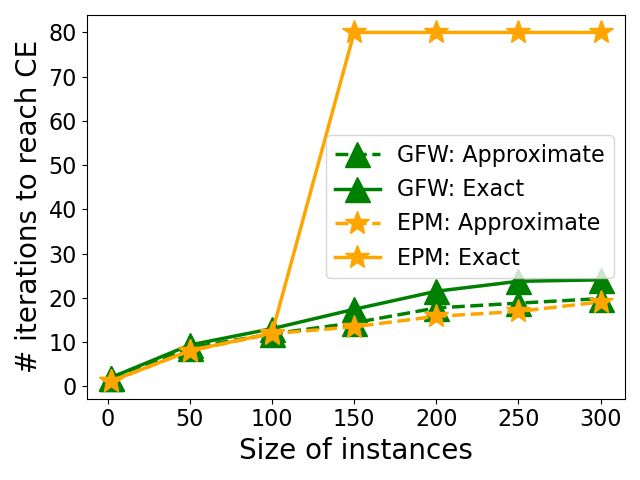
\includegraphics[width=0.28\linewidth]{ni_uniform.png}
    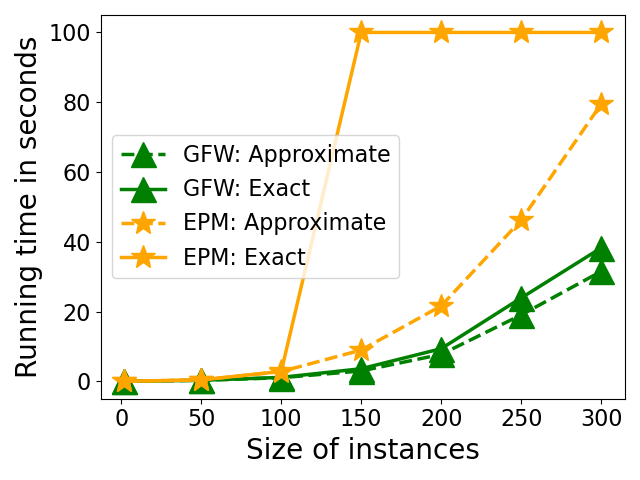
\includegraphics[width=0.28\linewidth]{rt_uniform.png}
    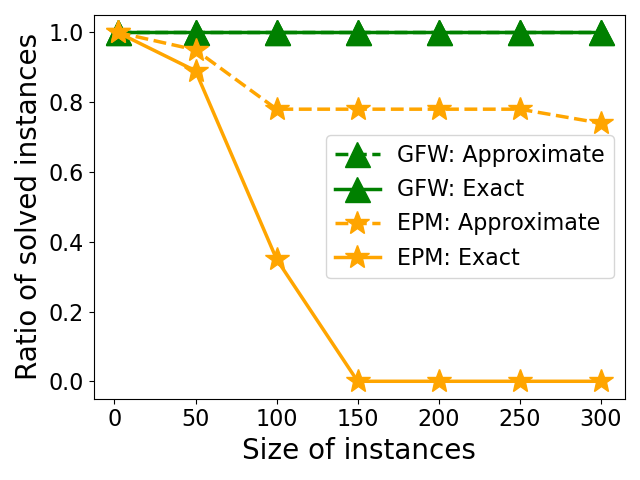
\includegraphics[width=0.28\linewidth]{sr_uniform.png}
    \makebox[0pt][r]{\makebox[30pt]{\raisebox{40pt}{\rotatebox[origin=c]{90}{lognormal}}}}%
    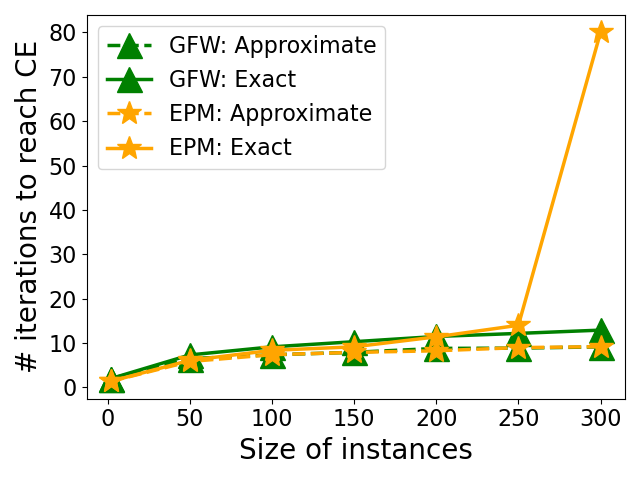
\includegraphics[width=0.28\linewidth]{ni_lognormal.png}
    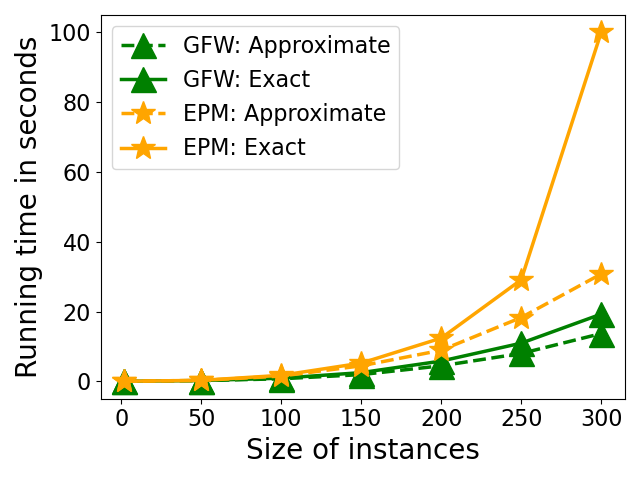
\includegraphics[width=0.28\linewidth]{rt_lognormal.png}
    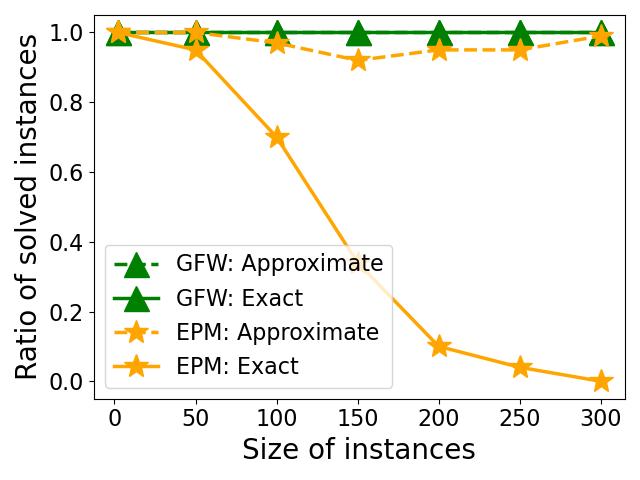
\includegraphics[width=0.28\linewidth]{sr_lognormal.png}
    \makebox[0pt][r]{\makebox[30pt]{\raisebox{40pt}{\rotatebox[origin=c]{90}{truncated normal}}}}%
    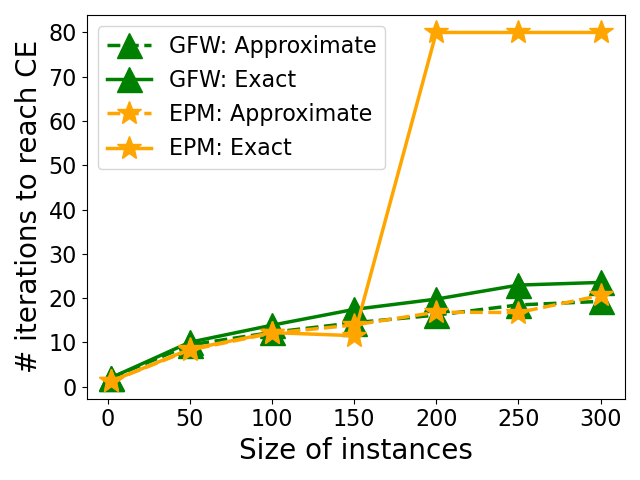
\includegraphics[width=0.28\linewidth]{ni_truncnormal.png}
    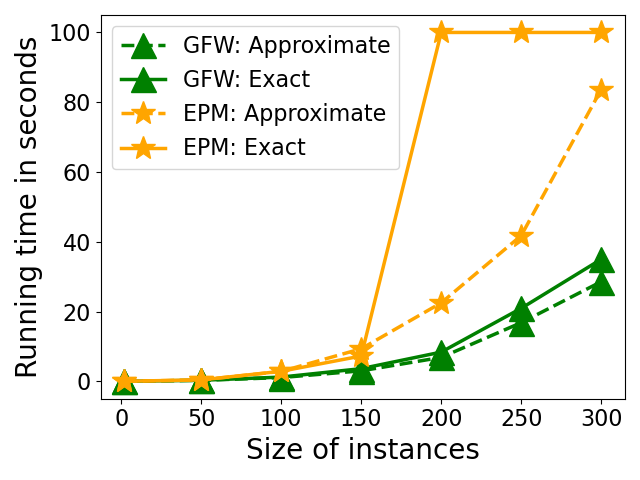
\includegraphics[width=0.28\linewidth]{rt_truncnormal.png}
    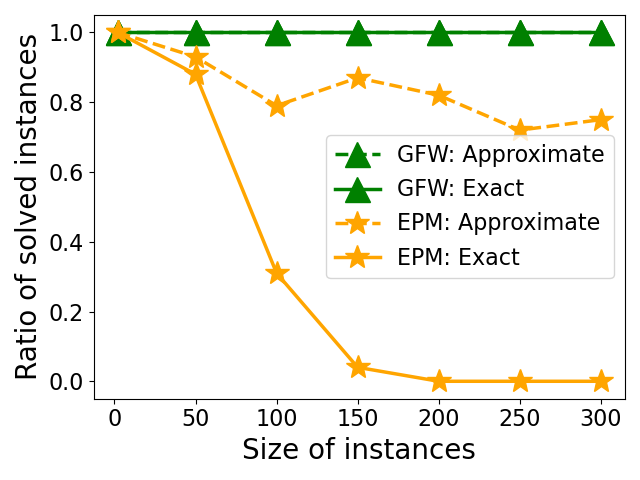
\includegraphics[width=0.28\linewidth]{sr_truncnormal.png}
    \makebox[0pt][r]{\makebox[30pt]{\raisebox{40pt}{\rotatebox[origin=c]{90}{exponential}}}}%
    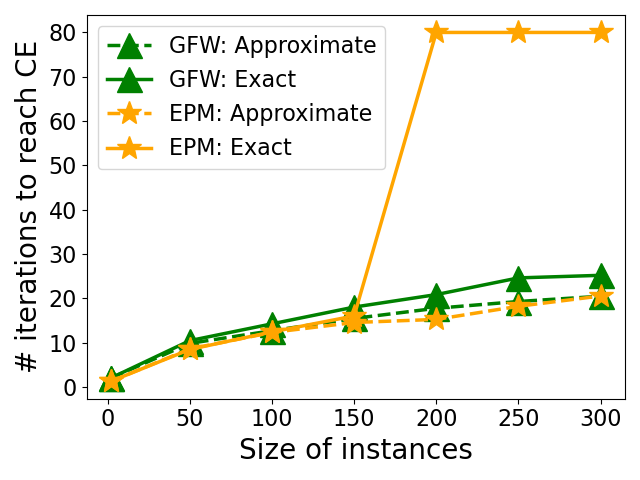
\includegraphics[width=0.28\linewidth]{ni_exponential.png}
    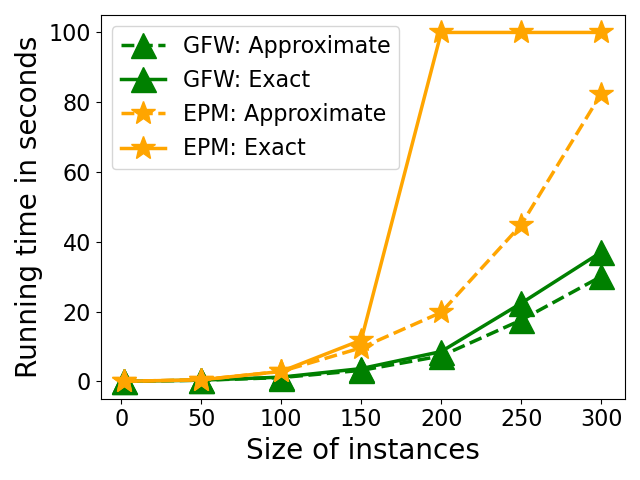
\includegraphics[width=0.28\linewidth]{rt_exponential.png}
    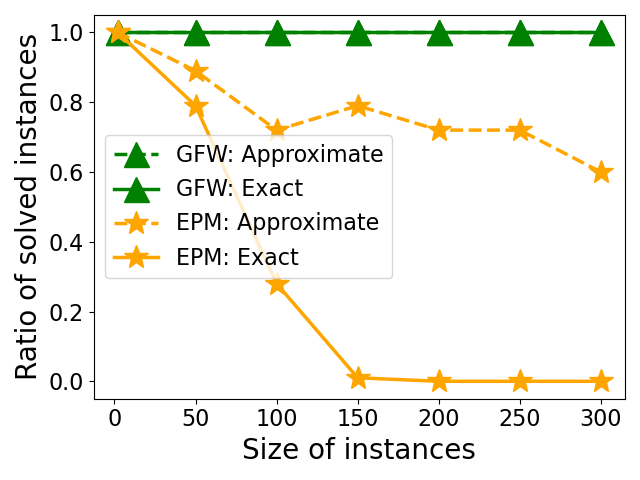
\includegraphics[width=0.28\linewidth]{sr_exponential.png}
    \makebox[0pt][r]{\makebox[30pt]{\raisebox{40pt}{\rotatebox[origin=c]{90}{randint(1,1000)}}}}%
    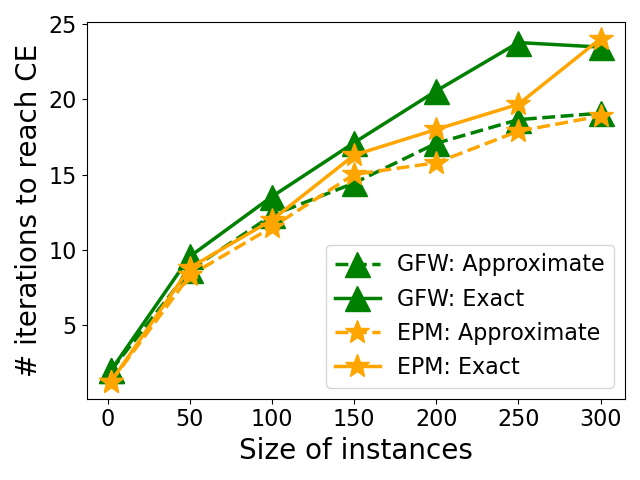
\includegraphics[width=0.28\linewidth]{ni_randint.png}
    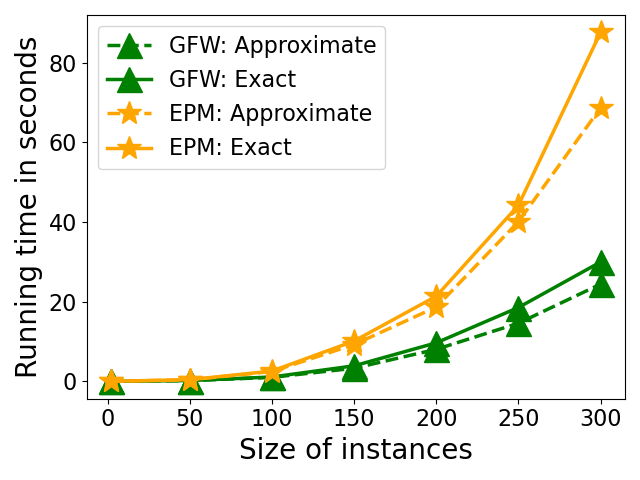
\includegraphics[width=0.28\linewidth]{rt_randint.png}
    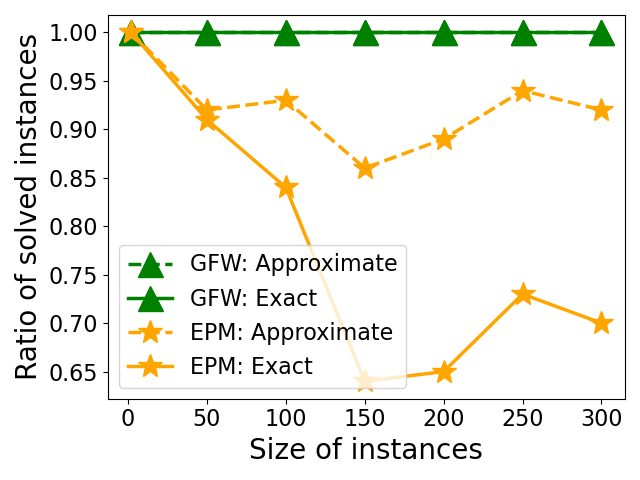
\includegraphics[width=0.28\linewidth]{sr_randint.png}
    \caption{Numerical results on iid randomly generated disutility matrix instances. 
    Each row corresponds to a different disutility distribution (noted on the left).
    Left: Average number of iterations to solve a given instance size.
    Middle: Average wall clock running time to solve a given instance size (using Gurobi for both algorithms).  
    Right: Fraction of instances solved for each algorithm. 
    GFW solves every instance for every distribution. 
    }
    \label{fig:random chores}
\end{figure}
In the left column of plots, we show the average number of iterations taken for each algorithm before finding a solution.
In the middle column of plots, we show the mean running time.
For both the left and middle column of plots, we only average over instances that were solved by EPM (and if EPM reaches the largest number on the y axis it denotes that  no instances were solved at a given size).
The right column shows the fraction of instances solved for each instance size.

In terms of the number of iterations taken by each algorithm, we see that that they are very comparable: in all cases where both algorithms solve some instances, the number of iterations is quite low: always below 30 iterations. When it does work, the EPM seems to take slightly fewer iterations than GFW in some cases.
In terms of runtime, GFW is generally faster than EPM: in every case where EPM solves at least one instance, we have the GFW is faster, sometimes by a factor of 2-4.
By far the most important result in terms of practicality is the right column of plots. We see that GFW successfully solves every instance we tried, out of the 3500 instances generated in total.
In contrast, EPM fails on a significant number of instances, sometimes failing on every instance for larger instance sizes, when attempting to compute exact CE.

The results on our semi-synthetic AAMAS bidding instances are shown in \cref{fig:bidding-data-sampled}.
Again we see that the number of iterations to reach CE is quite comparable across GFW and EPM, on the instances where EPM succeeds. The running time results are also similar: both for exact and approximate CE, GFW is faster than EPM in both the original data setting, and the added-noise setting. Notably, both algorithms are very fast, terminating in less than ten seconds for the original data, and GFW still terminates in less than 15 seconds for the added-noise setting.
On the original data, both algorithms solve every instance. This is likely due to the fact that the original data is a very special type of instance: there are only 5 possible distinct disutility values, and every buyer has a lot of chores with value 1. Thus, the equilibrium is very simple, which is also evident in the fact that the mean number of iterations is 3.5 even for the largest instances.
On the added-noise data, we see again that EPM exhibits significant numerical issues, failing on a large fraction of instances, especially for exact CE.

Overall, we conclude that GFW is the first highly practical algorithm: it solves every instance in very little time and in few iterations, even for instances where the size of the disutility matrix is $300\times 300$. In comparison, EPM fails to solve many instances in our datasets.
% \ntl{One reason: cannot find correct feasible allocation because the hyperplane is not accurate.} 
% \ntl{Another thing which is worth to mention is: to get an allocation corresponding to exact equilibrium, we need to solve an additional LP, which takes as much cost as the per-iteration LP solved in GFW.}
% \paragraph{Notations for EPM.} We define disutility space$+$ $\mathcal{D}^+$ as the space of all possible disutility profile corresponding to any allocation or over-allocation, i.e., 
% \begin{equation}
%     \mathcal{D}^+ = \left\{ d \in \mathbb{R}^n_{\geq 0} \;\vert\; \exists\; x \in \mathbb{R}^{n \times m}_{\geq 0} \mbox{ such that } d_i \geq \sum\nolimits_j d_{ij} x_{ij} \;\forall\; i \in [n], \sum\nolimits_i x_{ij} = 1 \;\forall\; j \in [m] \right\}. 
% \end{equation}
As discussed before, we do caution that the success of EPM is highly dependent on the performance of the Gurobi QP solver, and in particular its accuracy. We found that the QP performance of Gurobi can vary substantially across different machines, and unpredictably so.
% \ntl{To add some refrences. }
% the performance of Gurobi can be very different and unpredictable on different machines. 
For example, Gurobi may choose different methods to solve LPs or QPs based on how much RAM is available, as well as other factors. 
Due to this so-called "performance variability", it is difficult to conclusively evaluate the wall-clock performance of the algorithms, as both algorithms rely on the performance of Gurobi on large-size instances. 
In particular, some preliminary experiments suggests that the wall-clock performance of EPM improves relative to the wall-clock performance of GFW if one adds more RAM.
However, we found that even in this case, EPM still has a significant failure rate, since Gurobi still outputs approximate QP solutions, and this still leads to numerical errors that break EPM.


% \ntl{Careful Explanations.}










% \begin{figure}
%     \centering
%     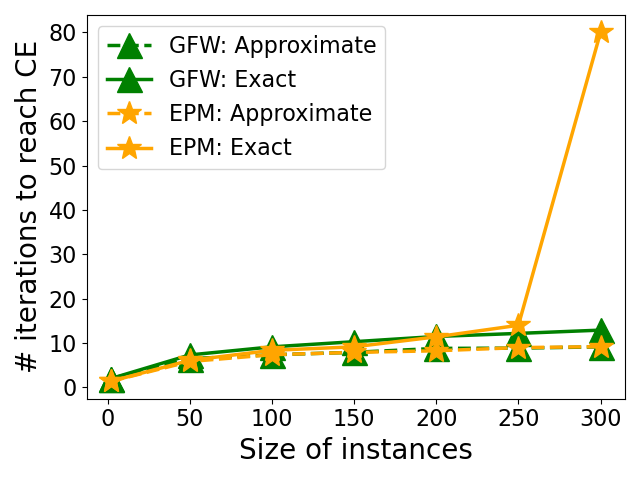
\includegraphics[width=0.32\linewidth]{ni_lognormal.png}
%     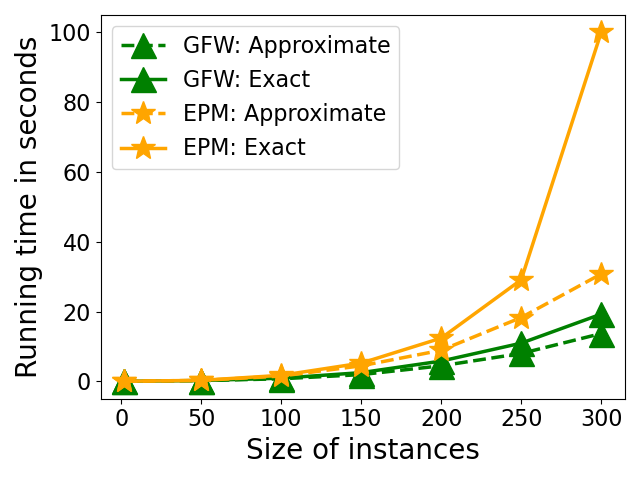
\includegraphics[width=0.32\linewidth]{rt_lognormal.png}
%     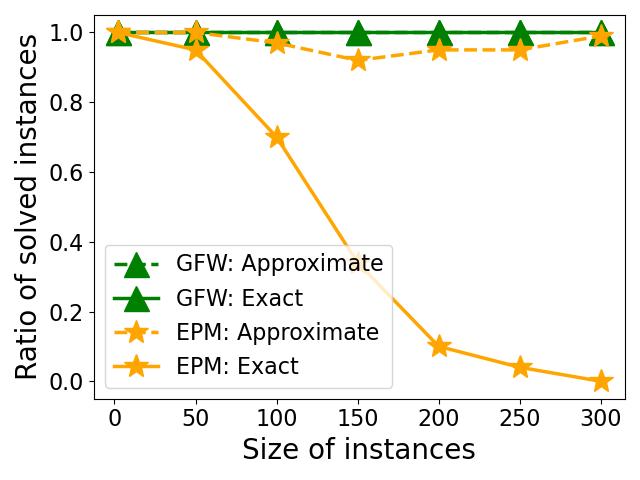
\includegraphics[width=0.32\linewidth]{sr_lognormal.png}
%     \caption{Numerical results on randomly generated log-normally distributed matrix instances. (To be changed)
%     All other settings are the same as~\cref{fig:uniform}. 
%     }
%     \label{fig:lognormal}
% \end{figure}

% \begin{figure}
%     \centering
%     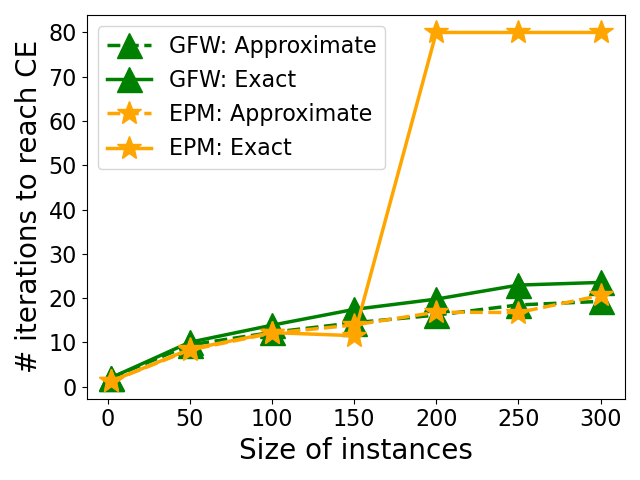
\includegraphics[width=0.32\linewidth]{ni_truncnormal.png}
%     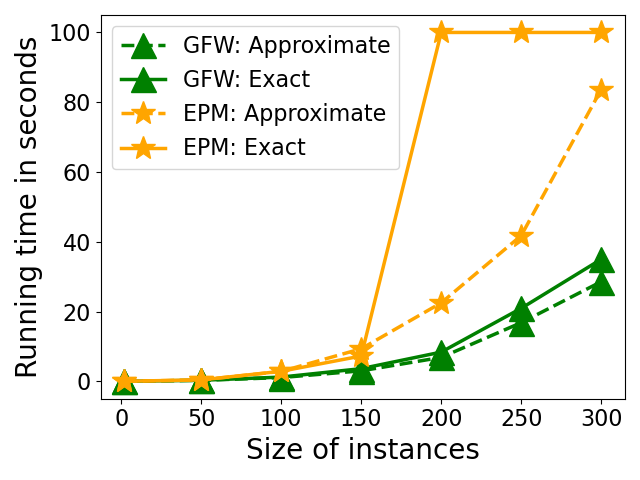
\includegraphics[width=0.32\linewidth]{rt_truncnormal.png}
%     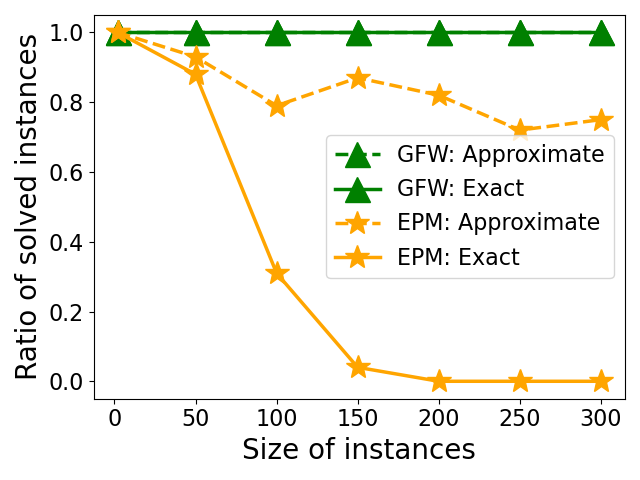
\includegraphics[width=0.32\linewidth]{sr_truncnormal.png}
%     \caption{Numerical results on randomly generated truncated normally (Gaussian) distributed matrix instances. 
%     All other settings are the same as~\cref{fig:uniform}. 
%     }
%     \label{fig:lognormal}
% \end{figure}

% \begin{figure}
%     \centering
%     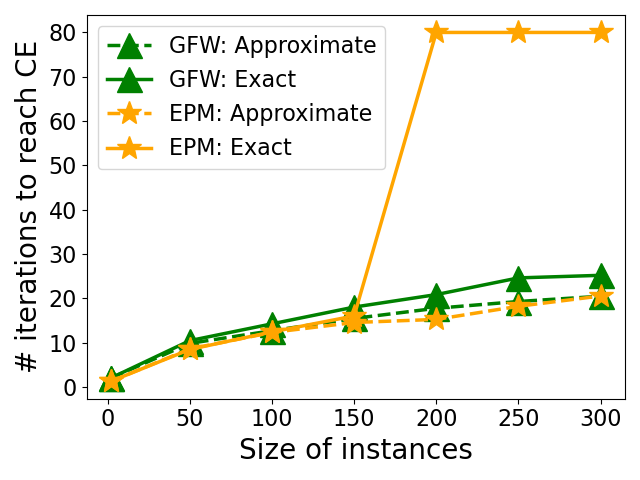
\includegraphics[width=0.32\linewidth]{ni_exponential.png}
%     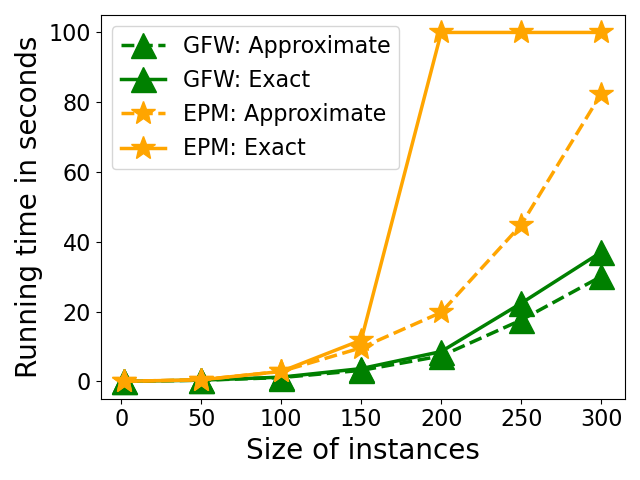
\includegraphics[width=0.32\linewidth]{rt_exponential.png}
%     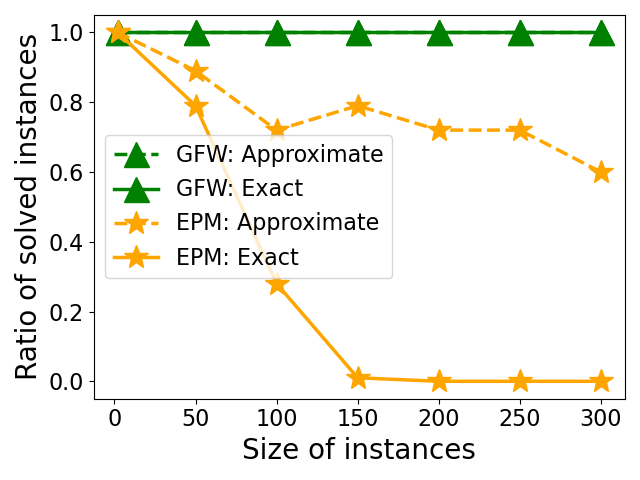
\includegraphics[width=0.32\linewidth]{sr_exponential.png}
%     \caption{Numerical results on randomly generated exponentially distributed matrix instances. 
%     All other settings are the same as~\cref{fig:uniform}. 
%     }
%     \label{fig:lognormal}
% \end{figure}

% \begin{figure}
%     \centering
%     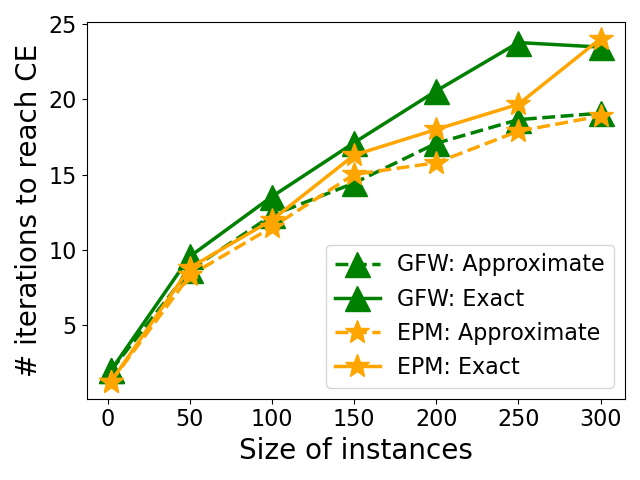
\includegraphics[width=0.32\linewidth]{ni_randint.png}
%     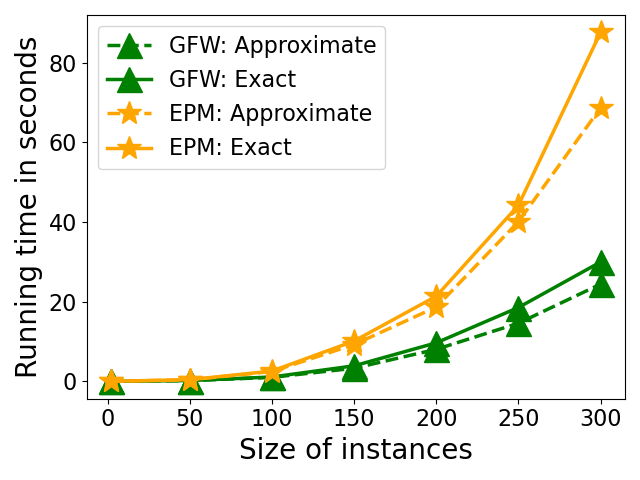
\includegraphics[width=0.32\linewidth]{rt_randint.png}
%     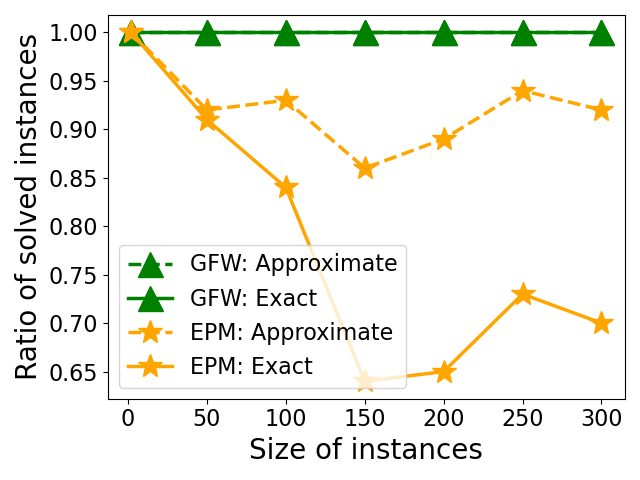
\includegraphics[width=0.32\linewidth]{sr_randint.png}
%     \caption{Numerical results on randomly generated integer (1 - 1000) matrix instances. 
%     All other settings are the same as~\cref{fig:uniform}.} 
%     \label{fig:randint}
% \end{figure}

\begin{figure}
    \centering
    \makebox[0pt][r]{\makebox[10pt]{\raisebox{40pt}{\rotatebox[origin=c]{90}{original}}}}%
    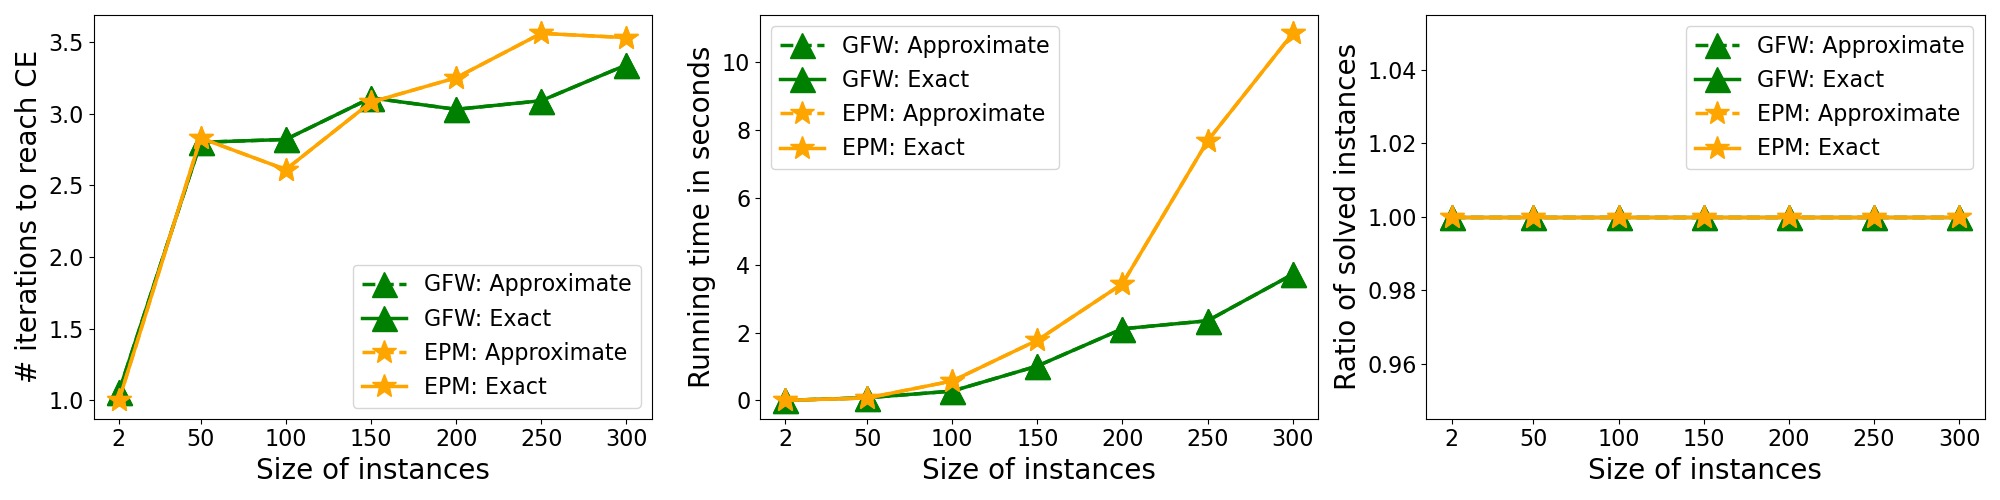
\includegraphics[width=0.85\linewidth]{bidding_data_int.png}
    \makebox[0pt][r]{\makebox[10pt]{\raisebox{40pt}{\rotatebox[origin=c]{90}{with noise}}}}%
    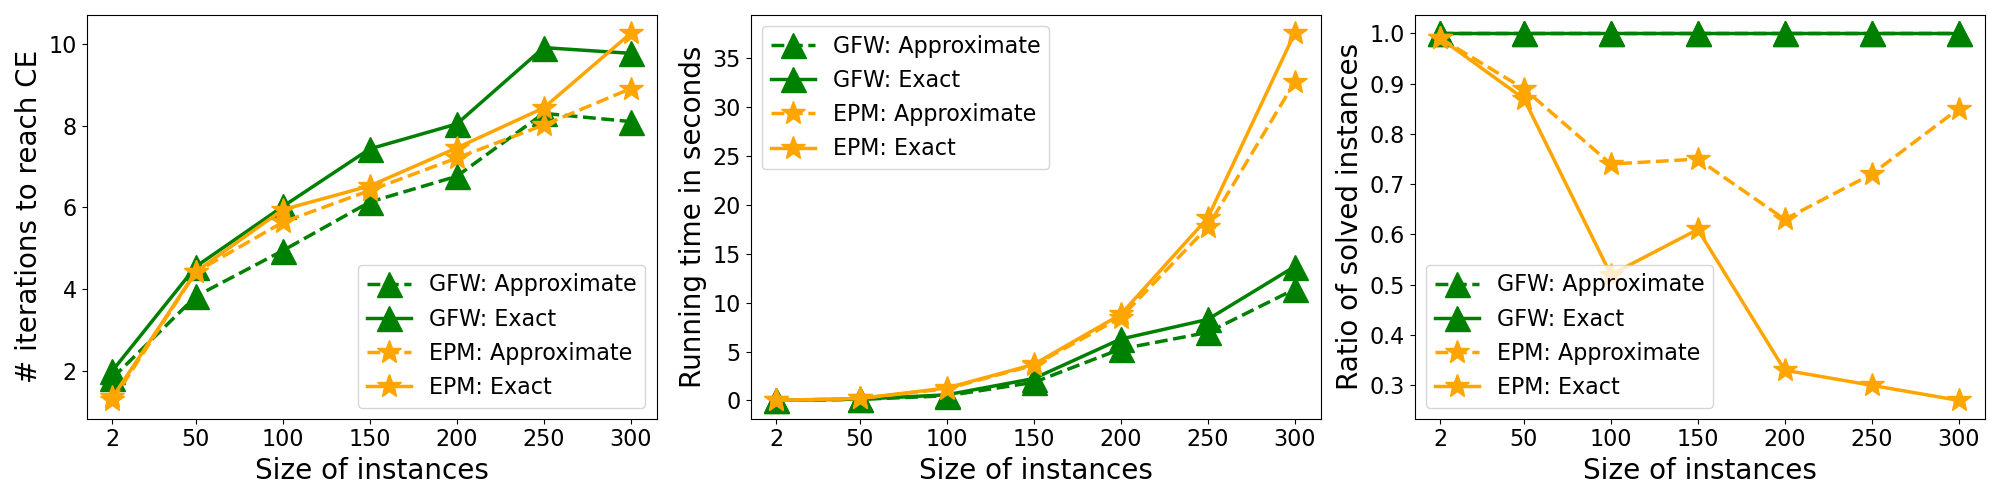
\includegraphics[width=0.85\linewidth]{bidding_data_with_noise_int.png}
    \caption{Numerical results on AAMAS PC member bidding data. 
    The top row uses the ``original'' valuations.
    The bottom row adds Gaussian noise.
    Left: Average number of iterations to solve a given instance size.
    Middle:  Average wall clock running time to solve a given instance size.
    Right: Fraction of instances solved.
    }
    \label{fig:bidding-data-sampled}
\end{figure}

% \begin{figure}
%     \centering
%     
\includegraphics[width=1\linewidth]{plots/bidding_data_with_noise_int.png}
%     \caption{Numerical results on sampled bidding data with normal noise.}
%     \label{fig:bidding-data-sampled-with-noise}
% \end{figure}


% \ck{Define what it means to "fail" in EPM: even small numerical error in Gurobi can lead to large error in the EPM.}


% \ck{AAMAS data plots:
% \begin{enumerate}
%     \item Wall-clock time for GFW and EPM
%     \item Number of iterations (if an algo fails, give highest number)
%     \item X axis: instance size (50, 100, 200, 300, 400, full dataset)
% \end{enumerate}
% }

%\section{Approximate CEEI and exact CEEI can be far apart}
%\ck{Move this to the end as part of a discussion on what's the challenge in going from approximate to exact CE?}


\section{Conclusion and Discussion}
We develop a new convex maximization program for computing CE in Fisher markets with chores, and showed that it satisfies some dual-like properties with the concave minimization program for computing CE.
We then derived a new redundant constraint which allows us to avoid directions that lead to infinitely positive objective. This yielded the first mathematical program for finding CE for chores such that it is possible to run iterative optimization methods over a convex feasible region.
We then introduced the GFW method for computing CE. From prior results on convex maximization over polytopes, it follows that this method terminates in a finite number of iterations. We then showed that, in fact, the method finds an $\epsilon$-approximate CE in $O(1/\epsilon^2$ iterations, while requiring only a simple LP solve at every iteration. We also gave a more general convergence result that generalizes prior results for strongly convex functions to Bregman-strongly-convex functions.
Finally, we showed through extensive numerical experiments that our method is highly practical: it solved every instance that we tried in a minute or less and is both robust and simple to implement. In contrast, we showed that the prior state-of-the-art method, the EPM, often fails to solve instances altogether, due to numerical accuracy problems that break the algorithm. 


\paragraph{Challenge of Moving from Approximate CE to Exact CE:} The obvious open problem is to settle the exact complexity of finding a CE in the chores market. A natural attempt would be to find a good approximate CE  and then argue how to move to a ``nearby'' exact CE. \emph{Unfortunately, such approaches can face the issue that there are instances where an approximate CE can be very far from an exact CE (See Section~\ref{example-CE} in Appendix for an example)}. 

Therefore, one may need to search for additional properties while looking out for a good approximate CE/ CEEI. Note that our GFW method indeed finds an exact CE in the chores market in finite time. In fact, it finds an exact CE in very few iterations in our experiments. Thus, it would be interesting to investigate instances where the time taken by GFW to reach an exact CE is exponential. We believe that this can improve our understanding of ``hard instances'' (if any) for iterative methods for computing a CE.

Despite the above hurdle, we believe that finding a $\varepsilon$-CE in the chores market with a better run time dependence on $1/\varepsilon$ is of theoretical interest. An ideal goal would be to have a poly-logarithmic dependence on $1/\varepsilon$, but any polynomial improvement would be a stepping stone (currently, all methods have a dependence of $\mathcal{O}(1/\varepsilon^2)$). 

\section*{Acknowledgments}
Christian Kroer was supported by the Office of Naval Research awards N00014-22-1-2530 and N00014-23-1-2374, and the National Science Foundation awards IIS-2147361 and IIS-2238960. Ruta Mehta was supported by NSF grant CCF-2334461 and NSF CAREER Award CCF-1750436. 

\bibliographystyle{plainnat}  
\bibliography{refs} 

\appendix
\section{A Primal-Dual Analysis of the Convergence of the Frank Wolfe Method to an Approximate Equilibrium}
\label{sec:primal-dual-convergence}
Since $f$ does not depend on $p$, we ease notation in this by section by writing $f(\beta)$ for the \ref{chores EG dual} objective function, which was previously defined as depending on both $p$ and $\beta$. 

Let $\{(p^t, \beta^t)\}_{t \geq 0}$ be the sequence of iterates generated by the greedy Frank Wolfe algorithm. Then, given $\beta^{t-1}_i$ for all $i\in [n]$, iteration $t$ of the Frank Wolfe algorithm attempts to find the vector $\beta^t$ such that 
\begin{equation}
\begin{aligned}
\min_{\beta} \quad & \sum_{i \in [n]} B_i \cdot \frac{\beta_i}{\beta^{t-1}_i}\\
\textrm{s.t.} \quad &  p_j - \beta_id_{ij} \leq 0  &\forall i,j\\
  &\quad  \sum_{j \in [m]} p_j =\sum_{i \in [n]}B_i = B    \\
  &\quad p_j \geq 0 &\forall j \\
  &\quad \beta_i \geq 0 &\forall i \\
\end{aligned}
\end{equation}

Let $x^t_{ij}$ be the optimal dual variable corresponding to the constraint $p_j - \beta_i d_{ij} \leq 0$, and $\delta^t$ be the optimal dual variable corresponding to the constraint $\sum_{j \in [m]}p_j = 1$ in the $t^{\mathit{th}}$ iteration of the greedy Frank Wolfe algorithm. 

\begin{claim}
\label{distutility-tech}
    For all $i \in [n]$, we have $\sum_{j \in [m]}d_{ij}x^t_{ij} = B_i/ \beta^{t-1}_i$. 
\end{claim}
\begin{proof}
    Under stationarity conditions of the optimum solutions, we have for all $i \in [n]$, $B_i/ \beta^{t-1}_i = \sum_{j \in [m]}d_{ij} x^t_{ij}$, whenever $\beta^t_i > 0$. Thus, it suffices to show that $\beta^t_i > 0$ for all $i \in [n]$. Assume otherwise, and $\beta^t_{\ell} = 0$. Since $\beta^t_{\ell} = \mathit{max}_{j \in [m]} p^t_{j}/d_{\ell j}$, this implies that $p^t_j = 0 $ for all $j \in [m]$, implying $\sum_{j \in [m]}p^t_j = 0$, which is a contradiction.
\end{proof}

We now make another technical observation. 
%By definition, $\beta^{t-1}$ was the optimum primal solution in the $(t-1)^{\mathit{th}}$ iteration of the algorithm. %Let $p'_j$, and $y_{ij}$, $\delta'$ denote the corresponding optimal prices and dual solutions for the previous iteration. Further, let $\beta'$ denote the optimal primal solution of the previous to previous iteration of the algorithm.

\begin{claim}
\label{disutilities-outflows}
    For all $i \in [n]$, we have  $\sum_{j \in [m]} d_{ij}x^{t-1}_{ij} = 1/\beta^{t-1}_i \cdot (\sum_{j \in [m]} p^{t-1}_j x^{t-1}_{ij}) $. Analogously, we have  $\sum_{j \in [m]} d_{ij}x^t_{ij} = 1/\beta^t_i \cdot (\sum_{j \in [m]} p^t_j x^t_{ij}) $.
\end{claim}

\begin{proof}
    Under the complementary slackness condition, we have 
    $x^{t-1}_{ij}(p^{t-1}_j - \beta^{t-1}_id_{ij} ) = 0$ for all $i,j$. Therefore, for each $i \in [n]$, we have 
    \begin{align*}
        &\sum_{j \in [m]}x^{t-1}_{ij}(p^{t-1}_j - \beta^{t-1}_id_{ij}) = 0\\
        &\implies \sum_{j \in [m]}p^{t-1}_j x^{t-1}_{ij} = \beta^{t-1}_i \sum_{j \in [m]} d_{ij}x^{t-1}_{ij} \\
        &\implies \sum_{j \in [m]} d_{ij}x^{t-1}_{ij} = 1/\beta^{t-1}_i \cdot (\sum_{j \in [m]} p^{t-1}_j x^{t-1}_{ij}) 
    \end{align*}
    The proof for the second statement of the theorem follows analogously.
\end{proof}
From Claim~\ref{disutilities-outflows}, it follows that $\prod_{i \in [n]} (\sum_{j \in [m]}d_{ij}x^{t-1}_{ij})^{B_i} = (\prod_{i \in [n]} (1/\beta^{t-1}_i) ^{B_i}) \cdot (\prod_{i \in [n]} (\sum_{j \in [m]}$  $p^{t-1}_j x^{t-1}_{ij})^{B_i})$ and Claim~\ref{distutility-tech} it follows that $\prod_{i \in [n]} (\sum_{j \in [m]}d_{ij}x^{t}_{ij})^{B_i} = \prod_{i \in [n]} (B_i/\beta^{t-1}_{i})^{B_i}$ . Therefore, if we comparing the weighted product of disutilities in the current iteration and the previous iteration, we have

\begin{align*}
  \frac{\prod_{i \in [n]} (\sum_{j \in [m]} d_{ij}x^t_{ij})^{B_i}}{\prod_{i \in [n]} (\sum_{j \in [m]} d_{ij}x^{t-1}_{ij})^{B_i}} &= \frac{\prod_{i \in [n]} (B_i/\beta^{t-1}_i)^{B_i}}{(\prod_{i \in [n]} (1/\beta^{t-1}_i)^{B_i} ) \cdot (\prod_{i \in [n]} (\sum_{j \in [m]}p^{t-1}_j x^{t-1}_{ij})^{B_i})}\\
  &= \frac{\prod_{i\in [n]} B_i^{B_i}}{\prod_{i \in [n]}(\sum_{j \in [m]}p^{t-1}_j x^{t-1}_{ij})^{B_i}}
\end{align*}

We now make an observation on $\sum_{i \in [n]}x^t_{ij}$-- interpreting the dual variables $x^t_{ij}$ as the fraction of chore $j$ allocated to agent $i$, one can interpret $\sum_{i \in [n]}x^t_{ij}$ as the total consumption of chore $j$ at the end of the $t^{\mathit{th}}$ iteration. %\BRC{Push  this sentence when we introduce dual variables?}

\begin{claim}
    \label{Allocation-claim}
    For all $i \in [n]$, and for all $t \geq 0$, we have $\sum_{i \in [n]} x^t_{ij} =  \frac{1}{B} \cdot \sum_{i \in [n]} B_i \cdot \frac{\beta^{t}_i}{\beta^{t-1}_i}$. %Similarly,  for all $i \in [n]$, we have $\sum_{i \in [n]} y_{ij} = \frac{1}{n} \cdot \sum_{i \in [n]} \frac{\beta_i}{\beta'_i}$
\end{claim}

\begin{proof}
    Under stationarity conditions, we have $\sum_{i \in [n]} x^t_{ij} = -\delta^t$ for all $j$ such that $p^t_j > 0$. Furthermore, from Claim~\ref{disutilities-outflows}, it follows that $\sum_{j \in [m]} p^t_j x^t_{ij} = \beta^t_i \cdot (\sum_{j \in [m]} d_{ij} x^t_{ij})$. Observe that,
    \begin{align*}
        \sum_{i \in [n]} B_i \cdot \frac{\beta^t_i}{\beta^{t-1}_i} &=\sum_{i \in [n]} \beta^t_i \cdot \frac{B_i}{\beta^{t-1}_i}\\ 
                                                  &= \sum_{i \in [n]} \beta^t_i \cdot (\sum_{j \in [m]} d_{ij}x^t_{ij})  &\text{(by Claim~\ref{distutility-tech})}\\
                                                  &= \sum_{i \in [n]} \sum_{j \in [m]} p^t_jx^t_{ij} &\text{(by Claim~\ref{disutilities-outflows})}\\
                                                  &= \sum_{j \in [m]} p^t_j \cdot \sum_{i \in [n]} x^t_{ij}\\
                                                      &= \sum_{j \mid p^t_j >0} p^t_j \cdot \sum_{i \in [n]} x^t_{ij}\\
                                                      &=\sum_{j \mid p^t_j >0} p^t_j \cdot (-\delta^t) = (-\delta^t) \cdot \sum_{j \in [m]} p^t_j\\
                                                      &=- (\sum_{i \in [n]} B_i)\delta^t = -B\delta^t
    \end{align*}
    Thus, we have $-\delta^t = \frac{1}{B} \cdot \sum_{i \in [n]} B_i \cdot \frac{\beta^t_i}{\beta^{t-1}_i}$. Therefore, for all $j \in [m]$, such that $p^t_j > 0$, we have $\sum_{i \in [n]} x^t_{ij} = - \delta^t = \frac{1}{B} \cdot \sum_{i \in [n]} B_i \cdot \frac{\beta^t_i}{\beta^{t-1}_i}$. It only suffices to show that $p^t_j > 0$ for all $j \in [m]$.
    
    We prove this by contradiction. Assume there exists a $j \in [m]$, such that $p^t_j = 0$. Then note that $p^t_j/d_{i j} < \beta^t_{i}$ for all $i \in [n]$ (follows from the fact that every $\beta^t_i$ is strictly positive). Note that there exists a $\gamma \ll  \mathit{min}_{\ell \in [n]} d_{\ell j} \beta^t_{\ell}$,  such that if we increase $p^t_j$ to $\gamma$, and decrease all other prices by a multiplicative factor of $(B-\gamma)$, we still have a feasible set of prices\footnote{All the prices are still non-negative and they still sum up to $B$.} and $\mathit{max}_{j \in [m]} p^t_j/d_{ij}$ strictly decreases for all $i \in [n]$. Let $\beta'_i = \mathit{max}_{j \in [m]} p^t_j/d_{ij}$ (post the multiplicative scaling). Note that $\beta'_i < \beta^t_i$ for all $i \in [n]$ and thus $\sum_{i \in [n]} B_i \cdot \beta'_i/\beta^{t-1}_i <\sum_{i\in [n]} B_i \cdot \beta^t_i/\beta^{t-1}_i$ which contradicts the optimality of $\beta^t$. 
\end{proof}

\begin{claim}
\label{progress}
If $( p^{t-1}, x^{t-1} )$ is not an $\varepsilon$-approximate equilibrium, then $\log \Bigg(\frac{\prod_{i\in [n]} B_i^{B_i}}{\prod_{i \in [n]}(\sum_{j \in [m]}p^{t-1}_j x^{t-1}_{ij})^{B_i}} \Bigg) \geq \min_i B_i \cdot \varepsilon^2/2.3$. 
\end{claim}

\begin{proof}
Note that $x^{t-1}_{ij} > 0$ only if $d_{ij}/p_j$ is minimum for all $j \in [m]$ for agent $i$. Thus, if $( p^{t-1}, x^{t-1} )$ is not an $\varepsilon$-approximate equilibrium, then there exists a $j \in [m]$ such that $\sum_{i \in [n]} x^{t-1}_{ij} < 1 - \varepsilon$, or there exists an $i \in [n]$, such that $|\sum_{j \in [m]} p^{t-1}_jx^{t-1}_{ij} - B_i| >  B_i\varepsilon$.

   \begin{itemize}
       \item \textbf{Case $\sum_{i \in [n]} x^{t-1}_{ij} < 1 - \varepsilon$:} From Claim~\ref{Allocation-claim}, it follows that $\sum_{i \in [n]} x^{t-1}_{ij} = \frac{1}{B} \cdot \sum_{i \in [n]} B_i\frac{\beta^{t-1}_i}{\beta^{t-2}_i} < 1 - \varepsilon$, implying that $\sum_{i \in [n]} B_i \frac{\beta^{t-1}_i}{\beta^{t-2}_i} < B(1 - \varepsilon)$. Further, observe that
       \begin{align*}
        \sum_{j \in [n]} p^{t-1}_j \cdot x^{t-1}_{ij} &= \beta^{t-1}_i \cdot \sum_{j \in [m]} d_{ij}x^{t-1}_{ij} &\text{(by Claim~\ref{disutilities-outflows})}\\
        &= \beta^{t-1}_i \cdot \frac{B_i}{\beta^{t-2}_i} &\text{(by Claim~\ref{distutility-tech})}
    \end{align*}
    Thus, we have $\sum_{i \in [n]} \sum_{j \in [m]} p^{t-1}_j x^{t-1}_{ij} = \sum_{i \in [n]} B_i \frac{\beta^{t-1}_i}{\beta^{t-2}_i} < B(1-\varepsilon)$. This implies that $\prod_{i \in [n]} (\sum_{j \in [m]} $ $ p^{t-1}_j x^{t-1}_{ij})^{B_i} \leq \prod_{i \in [n]} (B_i(1-\varepsilon))^{B_i}$, further implying that 
    \begin{align*}
        \frac{\prod_{i \in [n]} B_i^{B_i}}{\prod_{i \in [n]} (\sum_{j \in [m]} p^{t-1}_j x^{t-1}_{ij})^{B_i}} &\geq \frac{1}{(1-\varepsilon)^B}\\
                                                                   &\geq (1+\varepsilon)^B\\
                                                                   &\geq 1 + {B\varepsilon }
    \end{align*}
    Therefore, $\log \Bigg( \frac{\prod_{i \in [n]} B_i^{B_i}}{\prod_{i \in [n]} (\sum_{j \in [m]} p^{t-1}_j x^{t-1}_{ij})^{B_i}} \Bigg) \geq \log(1+B\varepsilon) \geq \min_i B_i \varepsilon^2/2.3$ as $\log(1+x) \geq x^2/2.3$ for all $x \in [0,1]$.

      \item \textbf{Case $|\sum_{j \in [m]} p^{t-1}_jx^{t-1}_{ij} - B_i| >  B_i\varepsilon$:}  %First note that if $\sum_{i \in [n]} \frac{\beta_i}{\beta'_i} < n(1-\varepsilon^2)$, we can use the same analysis from the above case, for our claim. So we assume otherwise. 
      Let $i$ be an agent such that $\sum_{j \in [m]} p^{t-1}_{j}x^{t-1}_{i j} = B_i(1 + \varepsilon')$, where $\varepsilon' \in \{-\theta, \theta \}$ for some $\theta > \varepsilon$. Observe that $\sum_{\ell \in [n] \setminus \{i\}} (\sum_{j \in [m]} p^{t-1}_jx^{t-1}_{ \ell j}) < B- B_i-B_i\varepsilon'$, as $\sum_{i \in [n]}(\sum_{j \in [m]} p^{t-1}_jx^{t-1}_{ij}) = \sum_{i \in [n]} B_i\frac{\beta^{t-1}_i}{\beta^{t-2}_i} \leq B$, and $\sum_{j \in [m]} p^{t-1}_{j}x^{t-1}_{i j} = B_i(1 + \varepsilon')$. This implies that $\prod_{\ell \in [n] \setminus \{i\}} (\sum_{j \in [m]} p^{t-1}_j x^{t-1}_{ \ell j})^{B_i} \leq \prod_{\ell \in [n] \setminus \{i\}} (B_{\ell} \cdot (1-\frac{B_i\varepsilon'}{B-B_i}))^{B_{\ell}}$. Before, we proceed, we mention the following useful fact,

      \begin{fact}
          \label{technical}
           For all real $x$, we have, $\log(e^x/(1+x)) \geq x^2/2.3$ for all $x \in [-1,1]$.
      \end{fact}
      
      We have,
      \begin{align*}
          \frac{\prod_{i \in [n]} B_i^{B_i}}{\prod_{i \in [n]} (\sum_{j \in [m]} p^{t-1}_j x^{t-1}_{ij})^{B_i}} &> \frac{\prod_{i \in [n]} B_i^{B_i}}{(B_i(1+\varepsilon'))^{B_i} \prod_{\ell \in [n] \setminus \{i\}} (B_{\ell} \cdot (1 - \frac{B_i\varepsilon'}{B-B_i}))^{B_{\ell}}}\\
                                                                    &=\frac{1}{(1 + \varepsilon')^{B_i} (1-\frac{B_i\varepsilon'}{B-B_i})^{(B-B_i)}}\\
                                                                    &\geq \frac{1}{(1 + \varepsilon')^{B_i} e^{-\frac{B_i\varepsilon'}{B-B_i} \cdot (B-B_i)}}\\        &= \frac{1}{(1 + \varepsilon')^{B_i}e^{-B_i\varepsilon'}}\\
                                                                    &=\bigg( \frac{1}{(1+\varepsilon')e^{-\varepsilon'}} \bigg)^{B_i} \qedhere
      \end{align*}
   \end{itemize}
\end{proof}
Now, observe that \
\begin{align*}
     \log \Bigg( \frac{\prod_{i \in [n]} B_i^{B_i}}{\prod_{i \in [n]} (\sum_{j \in [m]} p^{t-1}_j x^{t-1}_{ij})^{B_i}} \Bigg) &> \log \Bigg( \bigg(\frac{1}{(1+\varepsilon')e^{-\varepsilon'}}\bigg)^{B_i} \Bigg)\\
     &=B_i \log \Bigg(\frac{e^{\varepsilon'}}{1+\varepsilon'} \Bigg)\\
     &\geq B_i \frac{\varepsilon'^2}{2.3} &\text{(from Fact~\ref{technical})}\\
     &= \min_i B_i \frac{\theta^2}{2.3} = \min_i B_i \frac{\varepsilon^2}{2.3}. 
\end{align*}

We are now ready to prove our main result.

%\RM{The statement of the following theorem should convey the final result. Something like, Given a chores market, the GFW method converges to an $\epsilon$-approximate CE in $O(...)$ many steps. }
\begin{theorem}
\label{Theorem-convergence}
    Let $T \geq \frac{2.3(f(\beta^*) - f(\beta^0))}{\varepsilon^2 \min_i B_i }$. Then there exists a $t \leq T$, such that $(p^t,x^t)$ is a $\varepsilon$-CE 
\end{theorem}

\begin{proof}
    Assume otherwise, i.e., for all $t \in [T]$,  $(p^t,x^t)$ is not a $\varepsilon$-CE. Recall that we have,
    \begin{align*}
        \frac{\prod_{i \in [n]} (\sum_{j \in [m]} d_{ij}x^t_{ij})^{B_i}}{\prod_{i \in [n]} (\sum_{j \in [m]} d_{ij}x^{t-1}_{ij})^{B_i}} = \frac{\prod_{i \in [n]} B_i^{B_i} }{\prod_{i \in [n]}(\sum_{j \in [m]}p^{t-1}_j x^{t-1}_{ij})^{B_i}}
    \end{align*}
   By Claim~\ref{distutility-tech}, we can replace  $\sum_{j \in [m]} d_{ij}x^t_{ij}$ with $1/\beta^{t-1}_i$, implying,
   \begin{align}
       \label{eqn:prod-beta-comp}
        \frac{\prod_{i \in [n]} (1/\beta^{t-1}_i)^{B_i}}{\prod_{i \in [n]} (1/\beta^{t-2}_i)^{B_i}} = \frac{\prod_{i \in [n]} B_i^{B_i} }{\prod_{i \in [n]}(\sum_{j \in [m]}p^{t-1}_j x^{t-1}_{ij})^{B_i}}
    \end{align}
   Since $(p^{t-1},x^{t-1})$ is not a $\varepsilon$-CEEI, we have $ \log \bigg( \frac{\prod_{i \in [n]} B_i^{B_i} }{\prod_{i \in [n]}(\sum_{j \in [m]}p^{t-1}_j x^{t-1}_{ij})^{B_i}} \bigg) \geq \min_i B_i \cdot \varepsilon^2/2.3$ by Claim~\ref{progress}. Taking logs on both sides of Equation~\ref{eqn:prod-beta-comp}, we have
   \begin{align}
      \label{eq:beta-teslescoping}
       f(\beta^{t-1}) - f(\beta^{t-2})  \geq  \min_i B_i \cdot \varepsilon^2/2.3
   \end{align}
   Summing up Equation~\ref{eq:beta-teslescoping} from $t=2$ to $T+1$, we have $f(\beta^T) - f(\beta^0) > \min_i B_i \cdot T\varepsilon^2/2.3$. Since $f(\beta^*) \geq f(\beta^T)$, this implies that $f(\beta^*) - f(\beta^0) > \min_i B_i \cdot T\varepsilon^2/2.3$, implying that $T < 2.3(f(\beta^*) - f(\beta^0))/(\varepsilon^2 \cdot \min_i B_i)$, which is a contradiction. 
\end{proof}


\label{sec:polytime-conv-approxi} 


\section{Approximate CE and Exact CE can be far Apart}
\label{example-CE}
 We show that approximate CE and Exact CE can be far apart. Consider the following chores market: 2 agents $a_1$ and $a_2$, and 2 chores $c_1$ and $c_2$. Set $d_{11} = 1$, and $d_{12} = M$ for $M \gg 1$. Set $d_{21} = 1-\varepsilon$, and $d_{22} = 1 + \varepsilon$ for $\varepsilon \ll 1$. It is easy to verify that the only CEEI here is  
\begin{itemize}
    \item $p_1 = 2/(M+1)$ and $p_2 = 2M/(M+1)$,
    \item $x_{11} = 1$, $x_{21} = (M-1)/(2M)$, and 
    \item $x_{21} = 0$, and $x_{22} = (M+1)/(2M)$.
\end{itemize}

 Note that $\beta_1 = 2/(M+1)$, and $\beta_2 = 2M/((M+1)(1+\varepsilon))$. However, the following is an $\varepsilon$-approximate CEEI, with $\beta_1=\beta_2 = 1$, which is far from the only exact CEEI!

 \begin{itemize}
    \item $p_1 = 1-\varepsilon$ and $p_2 = 1+\varepsilon$,
    \item $x_{11} = 1-\varepsilon$, $x_{21} = 0$, and 
    \item $x_{21} = 0$, and $x_{22} = 1$.
\end{itemize}

\end{document} 